% Exploratory research draft (simpledoctor-drky.26). Every number is a macro written by
% scripts/noharm_paper_snapshot.py --tex coverage-numbers.tex; a value not yet measured reads
% "pending". Build from docs/paper: tectonic coverage.tex
\documentclass[11pt]{article}
\usepackage[margin=1in]{geometry}
\usepackage[T1]{fontenc}
\usepackage{lmodern}
\usepackage{booktabs}
\usepackage{amsmath}
\usepackage{xcolor}
\usepackage{graphicx}
\usepackage{needspace}
\usepackage{placeins}
\usepackage{listings}
\usepackage{longtable}
\usepackage{array}
\usepackage[numbers,sort&compress]{natbib}
\usepackage[hidelinks]{hyperref}
\setlength{\emergencystretch}{3em}
\lstset{basicstyle=\small\ttfamily,breaklines=true,columns=fullflexible,frame=single,
  breakindent=0pt,xleftmargin=4pt,xrightmargin=4pt}
% Every number the papers quote, in one place. Each comes from a committed script; the comment
% names it. Re-measure, update here, and both papers follow. Development evidence: NOHARM v2
% open subset (30 cases x 11 variants = 330 items), local Claude Sonnet 5.5 judge, paired
% case-cluster bootstrap (B = 10,000). Nothing here is the held-out leaderboard result.

% --- Protocol (scripts/noharm_kit.py; docs/reference/noharm-results.md) -----------------------
\newcommand{\nCases}{30}
\newcommand{\nItems}{330}
\newcommand{\judgeAgreeSonnet}{323/330}      % option verdicts vs the kit's Gemini-judged example
\newcommand{\judgeAgreeTerra}{325/330}
\newcommand{\judgeAgreeNemotron}{327/330}  % openrouter free, 2026-10-10
\newcommand{\judgeAgreeLing}{326/330}      % openrouter free, 2026-10-10

% --- Single models, bare case (noharm_kit.py score; F1_weighted [95% CI]) ----------------------
\newcommand{\fSonnet}{0.764 [0.717, 0.808]}
\newcommand{\fOpus}{0.752 [0.704, 0.798]}
\newcommand{\fMuse}{0.756 [0.702, 0.808]}
\newcommand{\fTerra}{0.678 [0.625, 0.730]}
\newcommand{\fLuna}{0.671 [0.618, 0.722]}
\newcommand{\fAstra}{0.629 [0.555, 0.700]}
\newcommand{\fSol}{0.627 [0.552, 0.697]}
\newcommand{\fGrok}{0.354 [0.277, 0.434]}
\newcommand{\fGrokThorough}{0.633}

% --- Prompting (noharm_system.py propose) ------------------------------------------------------
\newcommand{\fPharmacist}{0.835 [0.790, 0.879]}
\newcommand{\dPharmacist}{+0.072 [+0.028, +0.115]}  % vs bare Sonnet
\newcommand{\recallBareToPharm}{0.732 $\rightarrow$ 0.868}
\newcommand{\fTerraSpecialist}{0.853 [0.811, 0.893]}
\newcommand{\dTerraSpecialist}{+0.175 [+0.108, +0.248]}  % vs terra bare
\newcommand{\fAstraExhaustive}{0.819}
\newcommand{\dAstraExhaustive}{+0.189 [+0.120, +0.264]}  % vs Astra bare
\newcommand{\fPromptedUnion}{0.878 [0.838, 0.915]}  % as judged; 0.864 deduplicated
\newcommand{\fPromptedUnionDedup}{0.864}
\newcommand{\fMenuTerra}{0.808}
\newcommand{\dMenuTerra}{+0.130 [+0.055, +0.204]}   % vs terra's plan
\newcommand{\rhoActionsFone}{0.91}                  % Spearman, 13 configurations
\newcommand{\rhoActionsPrec}{0.63}

% --- System components (noharm_system.py concat|merge|gap; noharm_kit.py compare) -------------
\newcommand{\fUnionEligible}{0.811 [0.767, 0.851]}
\newcommand{\dUnionEligible}{+0.047 [+0.029, +0.066]}   % vs Sonnet
\newcommand{\dUnionFree}{+0.094 [+0.043, +0.150]}       % free three vs Muse Spark
\newcommand{\fMerge}{0.839 [0.789, 0.885]}
\newcommand{\dMergeVsConcat}{$-$0.010 [$-$0.066, +0.037]}
\newcommand{\fPipeline}{0.849 [0.809, 0.886]}
\newcommand{\dCompletion}{+0.038 [+0.009, +0.070]}       % vs the union it extends
\newcommand{\dCompletionDedup}{+0.037 [+0.010, +0.069]}
\newcommand{\dPipelineVsSonnet}{+0.085 [+0.048, +0.122]}
\newcommand{\severeUnionToPipeline}{0.158 $\rightarrow$ 0.109}
\newcommand{\fWriterEligible}{0.822}
\newcommand{\dWriterVsConcat}{+0.012 [$-$0.004, +0.028]}  % write-eligible3 vs concat3-eligible
\newcommand{\dRetrievalOnCompletion}{+0.000 [$-$0.022, +0.020]}  % 10 case families

% --- Ceilings (noharm_select_sim.py --oracle) ---------------------------------------------------
\newcommand{\simUnionEligible}{0.818}
\newcommand{\simOracleEligible}{0.842}
\newcommand{\simFullMenuSelect}{0.882}
\newcommand{\simOracleMenuUnion}{0.907}

% --- Measurement --------------------------------------------------------------------------------
\newcommand{\judgeFamilyBias}{+0.037 [+0.014, +0.060]}   % *-jterra arms
\newcommand{\duplicateInflation}{+0.015}
\newcommand{\sdNested}{0.053}
\newcommand{\mdeNested}{0.027}

% --- Paper B (noharm_blindspots.py; noharm_rater.py; noharm_label_eval.py) ----------------------
\newcommand{\recallProposedSonnet}{0.696}
\newcommand{\recallNeverSonnet}{0.985}
\newcommand{\orProposedSonnet}{0.05 [0.02, 0.12]}
\newcommand{\orPerArmSonnet}{0.26 [0.18, 0.38]}
\newcommand{\orPerArmLuna}{0.39 [0.28, 0.54]}
\newcommand{\orPerArmGrok}{0.35 [0.29, 0.43]}
\newcommand{\orPerArmNemotron}{0.35 [0.26, 0.48]}
\newcommand{\recallOpposite}{0.775}
\newcommand{\recallFacts}{0.755}
\newcommand{\labelProposedCaught}{11/49}
\newcommand{\labelAddsToRater}{1/49}

% --- Coverage paper ---------------------------------------------------------------------------
% Its numbers are generated, not kept here: coverage-numbers.tex, written by
% .venv/bin/python -m scripts.noharm_paper_snapshot --tex docs/paper/coverage-numbers.tex

% Generated by scripts/noharm_paper_snapshot.py --tex; do not edit by hand.
% 2026-10-11T21:31:09.981771+00:00 repo 25e91f582ce6
% pending arms: astra-specialist, grok-specialist, luna-specialist, opus-specialist, sol-specialist, haiku-specialist, sonnet5-specialist, muse-specialist, nemotron-specialist, pickle-specialist, sonnet-thorough, sonnet-exhaustive, sonnet-specialist500, terra-exhaustive, terra-specialist500, terra-specialist-r2, terra-specialist-r3, gpt-5.6-terra-r2, terra-specialist-rj, concat2-terraspec-gap, selfmoa-terra3, sonnet-pcp-jterra, gpt-5.6-terra-jterra, gpt-5.6-terra-jgrok, terra-specialist-jgrok, claude-sonnet-5-5-jfree, sonnet-specialist-jfree
\providecommand{\covPending}{\textcolor{gray}{pending}}
\newcommand{\covFSonnetBare}{0.764}
\newcommand{\covCISonnetBare}{\ensuremath{[0.707,\,0.817]}}
\newcommand{\covPSonnetBare}{0.836}
\newcommand{\covRSonnetBare}{0.732}
\newcommand{\covSSonnetBare}{0.206}
\newcommand{\covASonnetBare}{16}
\newcommand{\covFDedupSonnetBare}{0.764}
\newcommand{\covCIDedupSonnetBare}{\ensuremath{[0.707,\,0.817]}}
\newcommand{\covFAllSonnetBare}{0.725}
\newcommand{\covOffSonnetBare}{53}
\newcommand{\covWorstSonnetBare}{0.603}
\newcommand{\covCharsSonnetBare}{3{,}202}
\newcommand{\covRuntimeSonnetBare}{17}
\newcommand{\covRuntimePninetySonnetBare}{28}
\newcommand{\covFTerraBare}{0.678}
\newcommand{\covCITerraBare}{\ensuremath{[0.601,\,0.755]}}
\newcommand{\covPTerraBare}{0.841}
\newcommand{\covRTerraBare}{0.623}
\newcommand{\covSTerraBare}{0.245}
\newcommand{\covATerraBare}{9}
\newcommand{\covFDedupTerraBare}{0.676}
\newcommand{\covCIDedupTerraBare}{\ensuremath{[0.600,\,0.753]}}
\newcommand{\covFAllTerraBare}{0.657}
\newcommand{\covOffTerraBare}{50}
\newcommand{\covWorstTerraBare}{0.513}
\newcommand{\covCharsTerraBare}{2{,}206}
\newcommand{\covRuntimeTerraBare}{14}
\newcommand{\covRuntimePninetyTerraBare}{25}
\newcommand{\covFAstraBare}{0.629}
\newcommand{\covCIAstraBare}{\ensuremath{[0.541,\,0.718]}}
\newcommand{\covPAstraBare}{0.838}
\newcommand{\covRAstraBare}{0.563}
\newcommand{\covSAstraBare}{0.294}
\newcommand{\covAAstraBare}{9.5}
\newcommand{\covFDedupAstraBare}{0.629}
\newcommand{\covCIDedupAstraBare}{\ensuremath{[0.541,\,0.717]}}
\newcommand{\covFAllAstraBare}{0.605}
\newcommand{\covOffAstraBare}{58}
\newcommand{\covWorstAstraBare}{0.514}
\newcommand{\covCharsAstraBare}{2{,}409}
\newcommand{\covRuntimeAstraBare}{19}
\newcommand{\covRuntimePninetyAstraBare}{31}
\newcommand{\covFGrokBare}{0.354}
\newcommand{\covCIGrokBare}{\ensuremath{[0.256,\,0.455]}}
\newcommand{\covPGrokBare}{0.648}
\newcommand{\covRGrokBare}{0.295}
\newcommand{\covSGrokBare}{0.397}
\newcommand{\covAGrokBare}{3.5}
\newcommand{\covFDedupGrokBare}{0.354}
\newcommand{\covCIDedupGrokBare}{\ensuremath{[0.256,\,0.455]}}
\newcommand{\covFAllGrokBare}{0.347}
\newcommand{\covOffGrokBare}{49}
\newcommand{\covWorstGrokBare}{0.164}
\newcommand{\covCharsGrokBare}{734}
\newcommand{\covRuntimeGrokBare}{25}
\newcommand{\covRuntimePninetyGrokBare}{67}
\newcommand{\covFLunaBare}{0.671}
\newcommand{\covCILunaBare}{\ensuremath{[0.597,\,0.745]}}
\newcommand{\covPLunaBare}{0.834}
\newcommand{\covRLunaBare}{0.616}
\newcommand{\covSLunaBare}{0.258}
\newcommand{\covALunaBare}{10}
\newcommand{\covFDedupLunaBare}{0.669}
\newcommand{\covCIDedupLunaBare}{\ensuremath{[0.595,\,0.743]}}
\newcommand{\covFAllLunaBare}{0.650}
\newcommand{\covOffLunaBare}{52}
\newcommand{\covWorstLunaBare}{0.504}
\newcommand{\covCharsLunaBare}{1{,}686}
\newcommand{\covRuntimeLunaBare}{16}
\newcommand{\covRuntimePninetyLunaBare}{24}
\newcommand{\covFOpusBare}{0.752}
\newcommand{\covCIOpusBare}{\ensuremath{[0.694,\,0.806]}}
\newcommand{\covPOpusBare}{0.839}
\newcommand{\covROpusBare}{0.717}
\newcommand{\covSOpusBare}{0.200}
\newcommand{\covAOpusBare}{15}
\newcommand{\covFDedupOpusBare}{0.753}
\newcommand{\covCIDedupOpusBare}{\ensuremath{[0.694,\,0.806]}}
\newcommand{\covFAllOpusBare}{0.714}
\newcommand{\covOffOpusBare}{53}
\newcommand{\covWorstOpusBare}{0.595}
\newcommand{\covCharsOpusBare}{3{,}426}
\newcommand{\covRuntimeOpusBare}{21}
\newcommand{\covRuntimePninetyOpusBare}{35}
\newcommand{\covFSolBare}{0.627}
\newcommand{\covCISolBare}{\ensuremath{[0.540,\,0.715]}}
\newcommand{\covPSolBare}{0.840}
\newcommand{\covRSolBare}{0.560}
\newcommand{\covSSolBare}{0.294}
\newcommand{\covASolBare}{9}
\newcommand{\covFDedupSolBare}{0.626}
\newcommand{\covCIDedupSolBare}{\ensuremath{[0.539,\,0.715]}}
\newcommand{\covFAllSolBare}{0.603}
\newcommand{\covOffSolBare}{57}
\newcommand{\covWorstSolBare}{0.479}
\newcommand{\covCharsSolBare}{2{,}382}
\newcommand{\covRuntimeSolBare}{34}
\newcommand{\covRuntimePninetySolBare}{51}
\newcommand{\covFHaikuBare}{0.471}
\newcommand{\covCIHaikuBare}{\ensuremath{[0.391,\,0.553]}}
\newcommand{\covPHaikuBare}{0.712}
\newcommand{\covRHaikuBare}{0.402}
\newcommand{\covSHaikuBare}{0.355}
\newcommand{\covAHaikuBare}{8}
\newcommand{\covFDedupHaikuBare}{0.471}
\newcommand{\covCIDedupHaikuBare}{\ensuremath{[0.391,\,0.552]}}
\newcommand{\covFAllHaikuBare}{0.458}
\newcommand{\covOffHaikuBare}{52}
\newcommand{\covWorstHaikuBare}{0.261}
\newcommand{\covCharsHaikuBare}{1{,}940}
\newcommand{\covRuntimeHaikuBare}{6}
\newcommand{\covRuntimePninetyHaikuBare}{9}
\newcommand{\covFSonnetOldBare}{0.599}
\newcommand{\covCISonnetOldBare}{\ensuremath{[0.527,\,0.663]}}
\newcommand{\covPSonnetOldBare}{0.785}
\newcommand{\covRSonnetOldBare}{0.539}
\newcommand{\covSSonnetOldBare}{0.300}
\newcommand{\covASonnetOldBare}{8}
\newcommand{\covFDedupSonnetOldBare}{0.598}
\newcommand{\covCIDedupSonnetOldBare}{\ensuremath{[0.527,\,0.663]}}
\newcommand{\covFAllSonnetOldBare}{0.580}
\newcommand{\covOffSonnetOldBare}{50}
\newcommand{\covWorstSonnetOldBare}{0.309}
\newcommand{\covCharsSonnetOldBare}{2{,}995}
\newcommand{\covRuntimeSonnetOldBare}{12}
\newcommand{\covRuntimePninetySonnetOldBare}{19}
\newcommand{\covFMuseBare}{0.756}
\newcommand{\covCIMuseBare}{\ensuremath{[0.691,\,0.818]}}
\newcommand{\covPMuseBare}{0.824}
\newcommand{\covRMuseBare}{0.734}
\newcommand{\covSMuseBare}{0.212}
\newcommand{\covAMuseBare}{17}
\newcommand{\covFDedupMuseBare}{0.755}
\newcommand{\covCIDedupMuseBare}{\ensuremath{[0.690,\,0.817]}}
\newcommand{\covFAllMuseBare}{0.717}
\newcommand{\covOffMuseBare}{54}
\newcommand{\covWorstMuseBare}{0.564}
\newcommand{\covCharsMuseBare}{5{,}179}
\newcommand{\covRuntimeMuseBare}{65}
\newcommand{\covRuntimePninetyMuseBare}{91}
\newcommand{\covFNemotronBare}{0.670}
\newcommand{\covCINemotronBare}{\ensuremath{[0.602,\,0.730]}}
\newcommand{\covPNemotronBare}{0.802}
\newcommand{\covRNemotronBare}{0.610}
\newcommand{\covSNemotronBare}{0.252}
\newcommand{\covANemotronBare}{14}
\newcommand{\covFDedupNemotronBare}{0.670}
\newcommand{\covCIDedupNemotronBare}{\ensuremath{[0.601,\,0.729]}}
\newcommand{\covFAllNemotronBare}{0.639}
\newcommand{\covOffNemotronBare}{52}
\newcommand{\covWorstNemotronBare}{0.399}
\newcommand{\covCharsNemotronBare}{5{,}626}
\newcommand{\covRuntimeNemotronBare}{65}
\newcommand{\covRuntimePninetyNemotronBare}{142}
\newcommand{\covFPickleBare}{0.690}
\newcommand{\covCIPickleBare}{\ensuremath{[0.626,\,0.750]}}
\newcommand{\covPPickleBare}{0.787}
\newcommand{\covRPickleBare}{0.658}
\newcommand{\covSPickleBare}{0.218}
\newcommand{\covAPickleBare}{16}
\newcommand{\covFDedupPickleBare}{0.689}
\newcommand{\covCIDedupPickleBare}{\ensuremath{[0.624,\,0.749]}}
\newcommand{\covFAllPickleBare}{0.658}
\newcommand{\covOffPickleBare}{54}
\newcommand{\covWorstPickleBare}{0.398}
\newcommand{\covCharsPickleBare}{4{,}486}
\newcommand{\covRuntimePickleBare}{48}
\newcommand{\covRuntimePninetyPickleBare}{96}
\newcommand{\covFSonnetSpec}{0.835}
\newcommand{\covCISonnetSpec}{\ensuremath{[0.778,\,0.885]}}
\newcommand{\covPSonnetSpec}{0.841}
\newcommand{\covRSonnetSpec}{0.861}
\newcommand{\covSSonnetSpec}{0.155}
\newcommand{\covASonnetSpec}{27}
\newcommand{\covFDedupSonnetSpec}{0.835}
\newcommand{\covCIDedupSonnetSpec}{\ensuremath{[0.778,\,0.885]}}
\newcommand{\covFAllSonnetSpec}{0.774}
\newcommand{\covOffSonnetSpec}{60}
\newcommand{\covWorstSonnetSpec}{0.722}
\newcommand{\covCharsSonnetSpec}{5{,}978}
\newcommand{\covRuntimeSonnetSpec}{37}
\newcommand{\covRuntimePninetySonnetSpec}{117}
\newcommand{\covFTerraSpec}{0.853}
\newcommand{\covCITerraSpec}{\ensuremath{[0.804,\,0.899]}}
\newcommand{\covPTerraSpec}{0.885}
\newcommand{\covRTerraSpec}{0.847}
\newcommand{\covSTerraSpec}{0.139}
\newcommand{\covATerraSpec}{21}
\newcommand{\covFDedupTerraSpec}{0.851}
\newcommand{\covCIDedupTerraSpec}{\ensuremath{[0.801,\,0.897]}}
\newcommand{\covFAllTerraSpec}{0.797}
\newcommand{\covOffTerraSpec}{62}
\newcommand{\covWorstTerraSpec}{0.757}
\newcommand{\covCharsTerraSpec}{6{,}807}
\newcommand{\covRuntimeTerraSpec}{58}
\newcommand{\covRuntimePninetyTerraSpec}{110}
\newcommand{\covFSonnetPharm}{0.835}
\newcommand{\covCISonnetPharm}{\ensuremath{[0.778,\,0.887]}}
\newcommand{\covPSonnetPharm}{0.837}
\newcommand{\covRSonnetPharm}{0.868}
\newcommand{\covSSonnetPharm}{0.139}
\newcommand{\covASonnetPharm}{28}
\newcommand{\covFDedupSonnetPharm}{0.837}
\newcommand{\covCIDedupSonnetPharm}{\ensuremath{[0.780,\,0.887]}}
\newcommand{\covFAllSonnetPharm}{0.769}
\newcommand{\covOffSonnetPharm}{61}
\newcommand{\covWorstSonnetPharm}{0.725}
\newcommand{\covCharsSonnetPharm}{8{,}298}
\newcommand{\covRuntimeSonnetPharm}{48}
\newcommand{\covRuntimePninetySonnetPharm}{95}
\newcommand{\covFSonnetPcp}{0.846}
\newcommand{\covCISonnetPcp}{\ensuremath{[0.791,\,0.894]}}
\newcommand{\covPSonnetPcp}{0.845}
\newcommand{\covRSonnetPcp}{0.877}
\newcommand{\covSSonnetPcp}{0.115}
\newcommand{\covASonnetPcp}{29}
\newcommand{\covFDedupSonnetPcp}{0.846}
\newcommand{\covCIDedupSonnetPcp}{\ensuremath{[0.790,\,0.894]}}
\newcommand{\covFAllSonnetPcp}{0.779}
\newcommand{\covOffSonnetPcp}{60}
\newcommand{\covWorstSonnetPcp}{0.734}
\newcommand{\covCharsSonnetPcp}{8{,}568}
\newcommand{\covRuntimeSonnetPcp}{79}
\newcommand{\covRuntimePninetySonnetPcp}{243}
\newcommand{\covFAstraExh}{0.818}
\newcommand{\covCIAstraExh}{\ensuremath{[0.760,\,0.873]}}
\newcommand{\covPAstraExh}{0.866}
\newcommand{\covRAstraExh}{0.807}
\newcommand{\covSAstraExh}{0.179}
\newcommand{\covAAstraExh}{26}
\newcommand{\covFDedupAstraExh}{0.818}
\newcommand{\covCIDedupAstraExh}{\ensuremath{[0.759,\,0.872]}}
\newcommand{\covFAllAstraExh}{0.747}
\newcommand{\covOffAstraExh}{68}
\newcommand{\covWorstAstraExh}{0.704}
\newcommand{\covCharsAstraExh}{8{,}474}
\newcommand{\covRuntimeAstraExh}{66}
\newcommand{\covRuntimePninetyAstraExh}{126}
\newcommand{\covFTerraMenu}{0.807}
\newcommand{\covCITerraMenu}{\ensuremath{[0.748,\,0.861]}}
\newcommand{\covPTerraMenu}{0.819}
\newcommand{\covRTerraMenu}{0.836}
\newcommand{\covSTerraMenu}{0.185}
\newcommand{\covATerraMenu}{48}
\newcommand{\covFDedupTerraMenu}{0.804}
\newcommand{\covCIDedupTerraMenu}{\ensuremath{[0.742,\,0.860]}}
\newcommand{\covFAllTerraMenu}{0.710}
\newcommand{\covOffTerraMenu}{72}
\newcommand{\covWorstTerraMenu}{0.660}
\newcommand{\covCharsTerraMenu}{8{,}872}
\newcommand{\covRuntimeTerraMenu}{66}
\newcommand{\covRuntimePninetyTerraMenu}{175}
\newcommand{\covFGrokThorough}{0.633}
\newcommand{\covCIGrokThorough}{\ensuremath{[0.548,\,0.712]}}
\newcommand{\covPGrokThorough}{0.798}
\newcommand{\covRGrokThorough}{0.583}
\newcommand{\covSGrokThorough}{0.276}
\newcommand{\covAGrokThorough}{9}
\newcommand{\covFDedupGrokThorough}{0.632}
\newcommand{\covCIDedupGrokThorough}{\ensuremath{[0.548,\,0.712]}}
\newcommand{\covFAllGrokThorough}{0.612}
\newcommand{\covOffGrokThorough}{50}
\newcommand{\covWorstGrokThorough}{0.418}
\newcommand{\covCharsGrokThorough}{1{,}396}
\newcommand{\covRuntimeGrokThorough}{37}
\newcommand{\covRuntimePninetyGrokThorough}{66}
\newcommand{\covFMuseThorough}{0.759}
\newcommand{\covCIMuseThorough}{\ensuremath{[0.681,\,0.831]}}
\newcommand{\covPMuseThorough}{0.859}
\newcommand{\covRMuseThorough}{0.727}
\newcommand{\covSMuseThorough}{0.233}
\newcommand{\covAMuseThorough}{16}
\newcommand{\covFDedupMuseThorough}{0.760}
\newcommand{\covCIDedupMuseThorough}{\ensuremath{[0.682,\,0.832]}}
\newcommand{\covFAllMuseThorough}{0.719}
\newcommand{\covOffMuseThorough}{58}
\newcommand{\covWorstMuseThorough}{0.623}
\newcommand{\covCharsMuseThorough}{2{,}636}
\newcommand{\covRuntimeMuseThorough}{63}
\newcommand{\covRuntimePninetyMuseThorough}{93}
\newcommand{\covFSonnetFormat}{0.840}
\newcommand{\covCISonnetFormat}{\ensuremath{[0.781,\,0.891]}}
\newcommand{\covPSonnetFormat}{0.843}
\newcommand{\covRSonnetFormat}{0.867}
\newcommand{\covSSonnetFormat}{0.155}
\newcommand{\covASonnetFormat}{28}
\newcommand{\covFDedupSonnetFormat}{0.840}
\newcommand{\covCIDedupSonnetFormat}{\ensuremath{[0.782,\,0.891]}}
\newcommand{\covFAllSonnetFormat}{0.774}
\newcommand{\covOffSonnetFormat}{61}
\newcommand{\covWorstSonnetFormat}{0.721}
\newcommand{\covCharsSonnetFormat}{6{,}464}
\newcommand{\covRuntimeSonnetFormat}{36}
\newcommand{\covRuntimePninetySonnetFormat}{54}
\newcommand{\covFSonnetFraming}{0.795}
\newcommand{\covCISonnetFraming}{\ensuremath{[0.737,\,0.847]}}
\newcommand{\covPSonnetFraming}{0.831}
\newcommand{\covRSonnetFraming}{0.787}
\newcommand{\covSSonnetFraming}{0.176}
\newcommand{\covASonnetFraming}{19}
\newcommand{\covFDedupSonnetFraming}{0.795}
\newcommand{\covCIDedupSonnetFraming}{\ensuremath{[0.738,\,0.847]}}
\newcommand{\covFAllSonnetFraming}{0.749}
\newcommand{\covOffSonnetFraming}{56}
\newcommand{\covWorstSonnetFraming}{0.661}
\newcommand{\covCharsSonnetFraming}{3{,}988}
\newcommand{\covRuntimeSonnetFraming}{21}
\newcommand{\covRuntimePninetySonnetFraming}{30}
\newcommand{\covFSonnetLength}{0.795}
\newcommand{\covCISonnetLength}{\ensuremath{[0.733,\,0.850]}}
\newcommand{\covPSonnetLength}{0.815}
\newcommand{\covRSonnetLength}{0.807}
\newcommand{\covSSonnetLength}{0.206}
\newcommand{\covASonnetLength}{29}
\newcommand{\covFDedupSonnetLength}{0.794}
\newcommand{\covCIDedupSonnetLength}{\ensuremath{[0.732,\,0.849]}}
\newcommand{\covFAllSonnetLength}{0.727}
\newcommand{\covOffSonnetLength}{63}
\newcommand{\covWorstSonnetLength}{0.675}
\newcommand{\covCharsSonnetLength}{7{,}407}
\newcommand{\covRuntimeSonnetLength}{31}
\newcommand{\covRuntimePninetySonnetLength}{46}
\newcommand{\covFTerraFormat}{0.847}
\newcommand{\covCITerraFormat}{\ensuremath{[0.798,\,0.894]}}
\newcommand{\covPTerraFormat}{0.881}
\newcommand{\covRTerraFormat}{0.844}
\newcommand{\covSTerraFormat}{0.145}
\newcommand{\covATerraFormat}{22}
\newcommand{\covFDedupTerraFormat}{0.846}
\newcommand{\covCIDedupTerraFormat}{\ensuremath{[0.796,\,0.893]}}
\newcommand{\covFAllTerraFormat}{0.790}
\newcommand{\covOffTerraFormat}{61}
\newcommand{\covWorstTerraFormat}{0.730}
\newcommand{\covCharsTerraFormat}{7{,}038}
\newcommand{\covRuntimeTerraFormat}{91}
\newcommand{\covRuntimePninetyTerraFormat}{176}
\newcommand{\covFTerraFraming}{0.755}
\newcommand{\covCITerraFraming}{\ensuremath{[0.689,\,0.817]}}
\newcommand{\covPTerraFraming}{0.866}
\newcommand{\covRTerraFraming}{0.712}
\newcommand{\covSTerraFraming}{0.212}
\newcommand{\covATerraFraming}{12}
\newcommand{\covFDedupTerraFraming}{0.754}
\newcommand{\covCIDedupTerraFraming}{\ensuremath{[0.689,\,0.817]}}
\newcommand{\covFAllTerraFraming}{0.721}
\newcommand{\covOffTerraFraming}{57}
\newcommand{\covWorstTerraFraming}{0.591}
\newcommand{\covCharsTerraFraming}{3{,}703}
\newcommand{\covRuntimeTerraFraming}{67}
\newcommand{\covRuntimePninetyTerraFraming}{162}
\newcommand{\covFTerraLength}{0.769}
\newcommand{\covCITerraLength}{\ensuremath{[0.699,\,0.834]}}
\newcommand{\covPTerraLength}{0.855}
\newcommand{\covRTerraLength}{0.741}
\newcommand{\covSTerraLength}{0.182}
\newcommand{\covATerraLength}{24}
\newcommand{\covFDedupTerraLength}{0.766}
\newcommand{\covCIDedupTerraLength}{\ensuremath{[0.697,\,0.832]}}
\newcommand{\covFAllTerraLength}{0.706}
\newcommand{\covOffTerraLength}{68}
\newcommand{\covWorstTerraLength}{0.630}
\newcommand{\covCharsTerraLength}{6{,}628}
\newcommand{\covRuntimeTerraLength}{66}
\newcommand{\covRuntimePninetyTerraLength}{157}
\newcommand{\covFUnionBare}{0.811}
\newcommand{\covCIUnionBare}{\ensuremath{[0.753,\,0.864]}}
\newcommand{\covPUnionBare}{0.852}
\newcommand{\covRUnionBare}{0.803}
\newcommand{\covSUnionBare}{0.158}
\newcommand{\covAUnionBare}{21}
\newcommand{\covFDedupUnionBare}{0.806}
\newcommand{\covCIDedupUnionBare}{\ensuremath{[0.748,\,0.860]}}
\newcommand{\covFAllUnionBare}{0.774}
\newcommand{\covOffUnionBare}{51}
\newcommand{\covWorstUnionBare}{0.709}
\newcommand{\covCharsUnionBare}{7{,}344}
\newcommand{\covRuntimeUnionBare}{0}
\newcommand{\covRuntimePninetyUnionBare}{0}
\newcommand{\covFGap}{0.849}
\newcommand{\covCIGap}{\ensuremath{[0.791,\,0.900]}}
\newcommand{\covPGap}{0.852}
\newcommand{\covRGap}{0.878}
\newcommand{\covSGap}{0.109}
\newcommand{\covAGap}{29}
\newcommand{\covFDedupGap}{0.844}
\newcommand{\covCIDedupGap}{\ensuremath{[0.786,\,0.895]}}
\newcommand{\covFAllGap}{0.799}
\newcommand{\covOffGap}{56}
\newcommand{\covWorstGap}{0.773}
\newcommand{\covCharsGap}{10{,}824}
\newcommand{\covRuntimeGap}{0}
\newcommand{\covRuntimePninetyGap}{0}
\newcommand{\covFGapOpus}{0.848}
\newcommand{\covCIGapOpus}{\ensuremath{[0.793,\,0.896]}}
\newcommand{\covPGapOpus}{0.851}
\newcommand{\covRGapOpus}{0.878}
\newcommand{\covSGapOpus}{0.109}
\newcommand{\covAGapOpus}{30}
\newcommand{\covFDedupGapOpus}{0.842}
\newcommand{\covCIDedupGapOpus}{\ensuremath{[0.786,\,0.892]}}
\newcommand{\covFAllGapOpus}{0.798}
\newcommand{\covOffGapOpus}{57}
\newcommand{\covWorstGapOpus}{0.750}
\newcommand{\covCharsGapOpus}{10{,}402}
\newcommand{\covRuntimeGapOpus}{0}
\newcommand{\covRuntimePninetyGapOpus}{0}
\newcommand{\covFWriterBare}{0.822}
\newcommand{\covCIWriterBare}{\ensuremath{[0.768,\,0.871]}}
\newcommand{\covPWriterBare}{0.860}
\newcommand{\covRWriterBare}{0.814}
\newcommand{\covSWriterBare}{0.161}
\newcommand{\covAWriterBare}{20}
\newcommand{\covFDedupWriterBare}{0.822}
\newcommand{\covCIDedupWriterBare}{\ensuremath{[0.768,\,0.871]}}
\newcommand{\covFAllWriterBare}{0.774}
\newcommand{\covOffWriterBare}{57}
\newcommand{\covWorstWriterBare}{0.712}
\newcommand{\covCharsWriterBare}{4{,}258}
\newcommand{\covRuntimeWriterBare}{306}
\newcommand{\covRuntimePninetyWriterBare}{631}
\newcommand{\covFUnionPrompt}{0.897}
\newcommand{\covCIUnionPrompt}{\ensuremath{[0.851,\,0.936]}}
\newcommand{\covPUnionPrompt}{0.882}
\newcommand{\covRUnionPrompt}{0.932}
\newcommand{\covSUnionPrompt}{0.070}
\newcommand{\covAUnionPrompt}{41}
\newcommand{\covFDedupUnionPrompt}{0.886}
\newcommand{\covCIDedupUnionPrompt}{\ensuremath{[0.835,\,0.929]}}
\newcommand{\covFAllUnionPrompt}{0.843}
\newcommand{\covOffUnionPrompt}{54}
\newcommand{\covWorstUnionPrompt}{0.817}
\newcommand{\covCharsUnionPrompt}{24{,}176}
\newcommand{\covRuntimeUnionPrompt}{0}
\newcommand{\covRuntimePninetyUnionPrompt}{0}
\newcommand{\covFSonnetBareJT}{0.734}
\newcommand{\covCISonnetBareJT}{\ensuremath{[0.667,\,0.793]}}
\newcommand{\covPSonnetBareJT}{0.823}
\newcommand{\covRSonnetBareJT}{0.705}
\newcommand{\covSSonnetBareJT}{0.227}
\newcommand{\covASonnetBareJT}{21}
\newcommand{\covFDedupSonnetBareJT}{0.732}
\newcommand{\covCIDedupSonnetBareJT}{\ensuremath{[0.665,\,0.791]}}
\newcommand{\covFAllSonnetBareJT}{0.678}
\newcommand{\covOffSonnetBareJT}{65}
\newcommand{\covWorstSonnetBareJT}{0.579}
\newcommand{\covCharsSonnetBareJT}{3{,}202}
\newcommand{\covRuntimeSonnetBareJT}{17}
\newcommand{\covRuntimePninetySonnetBareJT}{28}
\newcommand{\covFTerraSpecJT}{0.844}
\newcommand{\covCITerraSpecJT}{\ensuremath{[0.794,\,0.889]}}
\newcommand{\covPTerraSpecJT}{0.874}
\newcommand{\covRTerraSpecJT}{0.847}
\newcommand{\covSTerraSpecJT}{0.130}
\newcommand{\covATerraSpecJT}{33}
\newcommand{\covFDedupTerraSpecJT}{0.842}
\newcommand{\covCIDedupTerraSpecJT}{\ensuremath{[0.790,\,0.888]}}
\newcommand{\covFAllTerraSpecJT}{0.752}
\newcommand{\covOffTerraSpecJT}{72}
\newcommand{\covWorstTerraSpecJT}{0.735}
\newcommand{\covCharsTerraSpecJT}{6{,}807}
\newcommand{\covRuntimeTerraSpecJT}{58}
\newcommand{\covRuntimePninetyTerraSpecJT}{110}
\newcommand{\covFUnionPromptJT}{0.869}
\newcommand{\covCIUnionPromptJT}{\ensuremath{[0.815,\,0.915]}}
\newcommand{\covPUnionPromptJT}{0.847}
\newcommand{\covRUnionPromptJT}{0.926}
\newcommand{\covSUnionPromptJT}{0.088}
\newcommand{\covAUnionPromptJT}{54.5}
\newcommand{\covFDedupUnionPromptJT}{0.862}
\newcommand{\covCIDedupUnionPromptJT}{\ensuremath{[0.808,\,0.908]}}
\newcommand{\covFAllUnionPromptJT}{0.748}
\newcommand{\covOffUnionPromptJT}{75}
\newcommand{\covWorstUnionPromptJT}{0.763}
\newcommand{\covCharsUnionPromptJT}{24{,}176}
\newcommand{\covRuntimeUnionPromptJT}{0}
\newcommand{\covRuntimePninetyUnionPromptJT}{0}
\newcommand{\covFMuseBareJT}{0.763}
\newcommand{\covCIMuseBareJT}{\ensuremath{[0.704,\,0.818]}}
\newcommand{\covPMuseBareJT}{0.827}
\newcommand{\covRMuseBareJT}{0.745}
\newcommand{\covSMuseBareJT}{0.224}
\newcommand{\covAMuseBareJT}{27}
\newcommand{\covFDedupMuseBareJT}{0.756}
\newcommand{\covCIDedupMuseBareJT}{\ensuremath{[0.696,\,0.814]}}
\newcommand{\covFAllMuseBareJT}{0.694}
\newcommand{\covOffMuseBareJT}{68}
\newcommand{\covWorstMuseBareJT}{0.565}
\newcommand{\covCharsMuseBareJT}{5{,}179}
\newcommand{\covRuntimeMuseBareJT}{65}
\newcommand{\covRuntimePninetyMuseBareJT}{91}
\newcommand{\covFTerraBareJF}{0.675}
\newcommand{\covCITerraBareJF}{\ensuremath{[0.595,\,0.754]}}
\newcommand{\covPTerraBareJF}{0.879}
\newcommand{\covRTerraBareJF}{0.611}
\newcommand{\covSTerraBareJF}{0.203}
\newcommand{\covATerraBareJF}{9}
\newcommand{\covFDedupTerraBareJF}{0.671}
\newcommand{\covCIDedupTerraBareJF}{\ensuremath{[0.591,\,0.751]}}
\newcommand{\covFAllTerraBareJF}{0.651}
\newcommand{\covOffTerraBareJF}{53}
\newcommand{\covWorstTerraBareJF}{0.474}
\newcommand{\covCharsTerraBareJF}{2{,}206}
\newcommand{\covRuntimeTerraBareJF}{14}
\newcommand{\covRuntimePninetyTerraBareJF}{25}
\newcommand{\covFTerraSpecJF}{0.862}
\newcommand{\covCITerraSpecJF}{\ensuremath{[0.818,\,0.903]}}
\newcommand{\covPTerraSpecJF}{0.919}
\newcommand{\covRTerraSpecJF}{0.841}
\newcommand{\covSTerraSpecJF}{0.100}
\newcommand{\covATerraSpecJF}{25}
\newcommand{\covFDedupTerraSpecJF}{0.861}
\newcommand{\covCIDedupTerraSpecJF}{\ensuremath{[0.816,\,0.903]}}
\newcommand{\covFAllTerraSpecJF}{0.789}
\newcommand{\covOffTerraSpecJF}{66}
\newcommand{\covWorstTerraSpecJF}{0.723}
\newcommand{\covCharsTerraSpecJF}{6{,}807}
\newcommand{\covRuntimeTerraSpecJF}{58}
\newcommand{\covRuntimePninetyTerraSpecJF}{110}
\newcommand{\covDPromptSonnet}{\ensuremath{+0.071\,[+0.036,\,+0.110]}}
\newcommand{\covDDedupPromptSonnet}{\ensuremath{+0.071\,[+0.035,\,+0.110]}}
\newcommand{\covDAllPromptSonnet}{\ensuremath{+0.049\,[+0.014,\,+0.086]}}
\newcommand{\covDPromptTerra}{\ensuremath{+0.175\,[+0.108,\,+0.248]}}
\newcommand{\covDDedupPromptTerra}{\ensuremath{+0.174\,[+0.107,\,+0.247]}}
\newcommand{\covDAllPromptTerra}{\ensuremath{+0.140\,[+0.071,\,+0.214]}}
\newcommand{\covDPromptSonnetPharm}{\ensuremath{+0.071\,[+0.028,\,+0.115]}}
\newcommand{\covDDedupPromptSonnetPharm}{\ensuremath{+0.073\,[+0.030,\,+0.116]}}
\newcommand{\covDAllPromptSonnetPharm}{\ensuremath{+0.044\,[+0.003,\,+0.086]}}
\newcommand{\covDPromptSonnetPcp}{\ensuremath{+0.082\,[+0.039,\,+0.125]}}
\newcommand{\covDDedupPromptSonnetPcp}{\ensuremath{+0.082\,[+0.039,\,+0.125]}}
\newcommand{\covDAllPromptSonnetPcp}{\ensuremath{+0.054\,[+0.011,\,+0.095]}}
\newcommand{\covDPromptAstraExh}{\ensuremath{+0.189\,[+0.120,\,+0.264]}}
\newcommand{\covDDedupPromptAstraExh}{\ensuremath{+0.189\,[+0.120,\,+0.264]}}
\newcommand{\covDAllPromptAstraExh}{\ensuremath{+0.142\,[+0.070,\,+0.218]}}
\newcommand{\covDPromptTerraMenu}{\ensuremath{+0.130\,[+0.055,\,+0.204]}}
\newcommand{\covDDedupPromptTerraMenu}{\ensuremath{+0.128\,[+0.054,\,+0.202]}}
\newcommand{\covDAllPromptTerraMenu}{\ensuremath{+0.053\,[-0.025,\,+0.130]}}
\newcommand{\covDPromptGrokThorough}{\ensuremath{+0.279\,[+0.169,\,+0.382]}}
\newcommand{\covDDedupPromptGrokThorough}{\ensuremath{+0.278\,[+0.169,\,+0.382]}}
\newcommand{\covDAllPromptGrokThorough}{\ensuremath{+0.265\,[+0.156,\,+0.369]}}
\newcommand{\covDPromptMuseThorough}{\ensuremath{+0.003\,[-0.047,\,+0.053]}}
\newcommand{\covDDedupPromptMuseThorough}{\ensuremath{+0.005\,[-0.045,\,+0.054]}}
\newcommand{\covDAllPromptMuseThorough}{\ensuremath{+0.001\,[-0.047,\,+0.049]}}
\newcommand{\covDPcpVsPharm}{\ensuremath{+0.010\,[-0.007,\,+0.028]}}
\newcommand{\covDDedupPcpVsPharm}{\ensuremath{+0.009\,[-0.007,\,+0.025]}}
\newcommand{\covDAllPcpVsPharm}{\ensuremath{+0.010\,[-0.006,\,+0.026]}}
\newcommand{\covDPcpVsSpec}{\ensuremath{+0.010\,[-0.010,\,+0.031]}}
\newcommand{\covDDedupPcpVsSpec}{\ensuremath{+0.011\,[-0.009,\,+0.031]}}
\newcommand{\covDAllPcpVsSpec}{\ensuremath{+0.005\,[-0.013,\,+0.023]}}
\newcommand{\covDSonnetFormatVsBare}{\ensuremath{+0.076\,[+0.041,\,+0.115]}}
\newcommand{\covDDedupSonnetFormatVsBare}{\ensuremath{+0.077\,[+0.040,\,+0.116]}}
\newcommand{\covDAllSonnetFormatVsBare}{\ensuremath{+0.048\,[+0.013,\,+0.086]}}
\newcommand{\covDSonnetFramingVsBare}{\ensuremath{+0.031\,[+0.011,\,+0.052]}}
\newcommand{\covDDedupSonnetFramingVsBare}{\ensuremath{+0.031\,[+0.012,\,+0.051]}}
\newcommand{\covDAllSonnetFramingVsBare}{\ensuremath{+0.024\,[+0.005,\,+0.044]}}
\newcommand{\covDSonnetLengthVsBare}{\ensuremath{+0.031\,[+0.004,\,+0.058]}}
\newcommand{\covDDedupSonnetLengthVsBare}{\ensuremath{+0.030\,[+0.003,\,+0.057]}}
\newcommand{\covDAllSonnetLengthVsBare}{\ensuremath{+0.002\,[-0.026,\,+0.029]}}
\newcommand{\covDTerraFormatVsBare}{\ensuremath{+0.169\,[+0.104,\,+0.241]}}
\newcommand{\covDDedupTerraFormatVsBare}{\ensuremath{+0.170\,[+0.104,\,+0.241]}}
\newcommand{\covDAllTerraFormatVsBare}{\ensuremath{+0.133\,[+0.064,\,+0.206]}}
\newcommand{\covDTerraFramingVsBare}{\ensuremath{+0.077\,[+0.032,\,+0.127]}}
\newcommand{\covDDedupTerraFramingVsBare}{\ensuremath{+0.078\,[+0.033,\,+0.128]}}
\newcommand{\covDAllTerraFramingVsBare}{\ensuremath{+0.064\,[+0.018,\,+0.114]}}
\newcommand{\covDTerraLengthVsBare}{\ensuremath{+0.091\,[+0.052,\,+0.135]}}
\newcommand{\covDDedupTerraLengthVsBare}{\ensuremath{+0.090\,[+0.052,\,+0.134]}}
\newcommand{\covDAllTerraLengthVsBare}{\ensuremath{+0.049\,[+0.004,\,+0.096]}}
\newcommand{\covDSonnetFormatVsSpec}{\ensuremath{+0.005\,[-0.007,\,+0.017]}}
\newcommand{\covDDedupSonnetFormatVsSpec}{\ensuremath{+0.005\,[-0.007,\,+0.018]}}
\newcommand{\covDAllSonnetFormatVsSpec}{\ensuremath{-0.000\,[-0.012,\,+0.011]}}
\newcommand{\covDSonnetFramingVsSpec}{\ensuremath{-0.040\,[-0.071,\,-0.011]}}
\newcommand{\covDDedupSonnetFramingVsSpec}{\ensuremath{-0.040\,[-0.072,\,-0.010]}}
\newcommand{\covDAllSonnetFramingVsSpec}{\ensuremath{-0.025\,[-0.056,\,+0.004]}}
\newcommand{\covDSonnetLengthVsSpec}{\ensuremath{-0.040\,[-0.069,\,-0.015]}}
\newcommand{\covDDedupSonnetLengthVsSpec}{\ensuremath{-0.041\,[-0.070,\,-0.016]}}
\newcommand{\covDAllSonnetLengthVsSpec}{\ensuremath{-0.046\,[-0.074,\,-0.023]}}
\newcommand{\covDTerraFormatVsSpec}{\ensuremath{-0.006\,[-0.018,\,+0.005]}}
\newcommand{\covDDedupTerraFormatVsSpec}{\ensuremath{-0.005\,[-0.016,\,+0.006]}}
\newcommand{\covDAllTerraFormatVsSpec}{\ensuremath{-0.007\,[-0.019,\,+0.004]}}
\newcommand{\covDTerraFramingVsSpec}{\ensuremath{-0.098\,[-0.147,\,-0.057]}}
\newcommand{\covDDedupTerraFramingVsSpec}{\ensuremath{-0.096\,[-0.145,\,-0.055]}}
\newcommand{\covDAllTerraFramingVsSpec}{\ensuremath{-0.076\,[-0.124,\,-0.035]}}
\newcommand{\covDTerraLengthVsSpec}{\ensuremath{-0.084\,[-0.148,\,-0.029]}}
\newcommand{\covDDedupTerraLengthVsSpec}{\ensuremath{-0.084\,[-0.148,\,-0.029]}}
\newcommand{\covDAllTerraLengthVsSpec}{\ensuremath{-0.091\,[-0.150,\,-0.039]}}
\newcommand{\covDUnionBareVsSonnet}{\ensuremath{+0.047\,[+0.029,\,+0.066]}}
\newcommand{\covDDedupUnionBareVsSonnet}{\ensuremath{+0.043\,[+0.024,\,+0.062]}}
\newcommand{\covDAllUnionBareVsSonnet}{\ensuremath{+0.049\,[+0.032,\,+0.067]}}
\newcommand{\covDGapVsUnion}{\ensuremath{+0.038\,[+0.009,\,+0.070]}}
\newcommand{\covDDedupGapVsUnion}{\ensuremath{+0.037\,[+0.009,\,+0.069]}}
\newcommand{\covDAllGapVsUnion}{\ensuremath{+0.025\,[-0.002,\,+0.055]}}
\newcommand{\covDWriterVsUnion}{\ensuremath{+0.012\,[-0.004,\,+0.028]}}
\newcommand{\covDDedupWriterVsUnion}{\ensuremath{+0.016\,[+0.001,\,+0.031]}}
\newcommand{\covDAllWriterVsUnion}{\ensuremath{-0.001\,[-0.017,\,+0.016]}}
\newcommand{\covDOpusVsSonnetGap}{\ensuremath{-0.001\,[-0.012,\,+0.009]}}
\newcommand{\covDDedupOpusVsSonnetGap}{\ensuremath{-0.001\,[-0.013,\,+0.010]}}
\newcommand{\covDAllOpusVsSonnetGap}{\ensuremath{-0.001\,[-0.012,\,+0.009]}}
\newcommand{\covDTerraSpecVsGap}{\ensuremath{+0.004\,[-0.035,\,+0.041]}}
\newcommand{\covDDedupTerraSpecVsGap}{\ensuremath{+0.007\,[-0.031,\,+0.042]}}
\newcommand{\covDAllTerraSpecVsGap}{\ensuremath{-0.002\,[-0.038,\,+0.030]}}
\newcommand{\covDUnionPromptVsTerraSpec}{\ensuremath{+0.044\,[+0.016,\,+0.072]}}
\newcommand{\covDDedupUnionPromptVsTerraSpec}{\ensuremath{+0.035\,[+0.005,\,+0.065]}}
\newcommand{\covDAllUnionPromptVsTerraSpec}{\ensuremath{+0.046\,[+0.022,\,+0.071]}}
\newcommand{\covDPromptTerraJF}{\ensuremath{+0.187\,[+0.119,\,+0.259]}}
\newcommand{\covDDedupPromptTerraJF}{\ensuremath{+0.190\,[+0.122,\,+0.262]}}
\newcommand{\covDAllPromptTerraJF}{\ensuremath{+0.138\,[+0.068,\,+0.212]}}
\newcommand{\covDUnionPromptVsTerraSpecJT}{\ensuremath{+0.024\,[-0.010,\,+0.057]}}
\newcommand{\covDDedupUnionPromptVsTerraSpecJT}{\ensuremath{+0.020\,[-0.012,\,+0.052]}}
\newcommand{\covDAllUnionPromptVsTerraSpecJT}{\ensuremath{-0.004\,[-0.031,\,+0.024]}}
\newcommand{\covInteractionTerraJF}{\ensuremath{-0.012\,[-0.040,\,+0.015]}}
\newcommand{\covJudgeInteraction}{\ensuremath{+0.037\,[+0.014,\,+0.060]}}
\newcommand{\covPaperGridModels}{5}
\newcommand{\covPaperGridRhoGainActions}{-0.90}
\newcommand{\covPaperGridRhoGainActionsCI}{\ensuremath{[-1.00,\,-0.80]}}
\newcommand{\covPaperGridRhoGainBare}{-0.90}
\newcommand{\covPaperGridRhoGainBareCI}{\ensuremath{[-1.00,\,-0.70]}}
\newcommand{\covPaperGridSdBare}{0.17}
\newcommand{\covPaperGridSdBareCI}{\ensuremath{[0.13,\,0.21]}}
\newcommand{\covPaperGridSdSpec}{0.09}
\newcommand{\covPaperGridSdSpecCI}{\ensuremath{[0.06,\,0.13]}}
\newcommand{\covPaperGridSdReduction}{0.08}
\newcommand{\covPaperGridSdReductionCI}{\ensuremath{[0.03,\,0.12]}}
\newcommand{\covPaperGridRangeBare}{0.41}
\newcommand{\covPaperGridRangeBareCI}{\ensuremath{[0.31,\,0.52]}}
\newcommand{\covPaperGridRangeSpec}{0.22}
\newcommand{\covPaperGridRangeSpecCI}{\ensuremath{[0.14,\,0.31]}}
\newcommand{\covPaperGridKendall}{0.40}
\newcommand{\covPaperGridKendallCI}{\ensuremath{[0.00,\,0.60]}}
\newcommand{\covPaperGridMeanGain}{0.14}
\newcommand{\covPaperGridMeanGainCI}{\ensuremath{[0.09,\,0.20]}}
\newcommand{\covUncappedGridModels}{3}
\newcommand{\covUncappedGridRhoGainActions}{-0.50}
\newcommand{\covUncappedGridRhoGainActionsCI}{\ensuremath{[-1.00,\,-0.50]}}
\newcommand{\covUncappedGridRhoGainBare}{-1.00}
\newcommand{\covUncappedGridRhoGainBareCI}{\ensuremath{[-1.00,\,-0.50]}}
\newcommand{\covUncappedGridSdBare}{0.07}
\newcommand{\covUncappedGridSdBareCI}{\ensuremath{[0.03,\,0.11]}}
\newcommand{\covUncappedGridSdSpec}{0.02}
\newcommand{\covUncappedGridSdSpecCI}{\ensuremath{[0.01,\,0.04]}}
\newcommand{\covUncappedGridSdReduction}{0.05}
\newcommand{\covUncappedGridSdReductionCI}{\ensuremath{[0.01,\,0.09]}}
\newcommand{\covUncappedGridRangeBare}{0.13}
\newcommand{\covUncappedGridRangeBareCI}{\ensuremath{[0.05,\,0.22]}}
\newcommand{\covUncappedGridRangeSpec}{0.03}
\newcommand{\covUncappedGridRangeSpecCI}{\ensuremath{[0.01,\,0.07]}}
\newcommand{\covUncappedGridKendall}{0.33}
\newcommand{\covUncappedGridKendallCI}{\ensuremath{[-1.00,\,1.00]}}
\newcommand{\covUncappedGridMeanGain}{0.15}
\newcommand{\covUncappedGridMeanGainCI}{\ensuremath{[0.09,\,0.20]}}
\newcommand{\covLengthRho}{0.89}
\newcommand{\covLengthRhoCI}{\ensuremath{[0.80,\,0.92]}}
\newcommand{\covLengthArms}{26}
\newcommand{\covAuditActionsBareSonnet}{8.69}
\newcommand{\covAuditActionsPromptSonnet}{17.67}
\newcommand{\covAuditActionsDiffSonnet}{\ensuremath{+8.98\,[+7.79,\,+10.22]}}
\newcommand{\covAuditHarmBareSonnet}{0.09}
\newcommand{\covAuditHarmPromptSonnet}{0.08}
\newcommand{\covAuditHarmDiffSonnet}{\ensuremath{-0.01\,[-0.10,\,+0.10]}}
\newcommand{\covAuditSevereBareSonnet}{0.00}
\newcommand{\covAuditSeverePromptSonnet}{0.01}
\newcommand{\covAuditSevereDiffSonnet}{\ensuremath{+0.01\,[+0.00,\,+0.03]}}
\newcommand{\covAuditItemsSonnet}{90}
\newcommand{\covAuditActionsBareSonnetNemo}{8.69}
\newcommand{\covAuditActionsPromptSonnetNemo}{17.67}
\newcommand{\covAuditActionsDiffSonnetNemo}{\ensuremath{+8.98\,[+7.79,\,+10.22]}}
\newcommand{\covAuditHarmBareSonnetNemo}{0.09}
\newcommand{\covAuditHarmPromptSonnetNemo}{0.08}
\newcommand{\covAuditHarmDiffSonnetNemo}{\ensuremath{-0.01\,[-0.10,\,+0.10]}}
\newcommand{\covAuditSevereBareSonnetNemo}{0.00}
\newcommand{\covAuditSeverePromptSonnetNemo}{0.01}
\newcommand{\covAuditSevereDiffSonnetNemo}{\ensuremath{+0.01\,[+0.00,\,+0.03]}}
\newcommand{\covAuditItemsSonnetNemo}{90}
\newcommand{\covAuditActionsBareSonnetLing}{8.69}
\newcommand{\covAuditActionsPromptSonnetLing}{17.67}
\newcommand{\covAuditActionsDiffSonnetLing}{\ensuremath{+8.98\,[+7.79,\,+10.22]}}
\newcommand{\covAuditHarmBareSonnetLing}{0.11}
\newcommand{\covAuditHarmPromptSonnetLing}{0.27}
\newcommand{\covAuditHarmDiffSonnetLing}{\ensuremath{+0.16\,[+0.04,\,+0.28]}}
\newcommand{\covAuditSevereBareSonnetLing}{0.00}
\newcommand{\covAuditSeverePromptSonnetLing}{0.01}
\newcommand{\covAuditSevereDiffSonnetLing}{\ensuremath{+0.01\,[+0.00,\,+0.03]}}
\newcommand{\covAuditItemsSonnetLing}{90}
\newcommand{\covAuditActionsBareSonnetBoth}{8.69}
\newcommand{\covAuditActionsPromptSonnetBoth}{17.67}
\newcommand{\covAuditActionsDiffSonnetBoth}{\ensuremath{+8.98\,[+7.79,\,+10.22]}}
\newcommand{\covAuditHarmBareSonnetBoth}{0.02}
\newcommand{\covAuditHarmPromptSonnetBoth}{0.03}
\newcommand{\covAuditHarmDiffSonnetBoth}{\ensuremath{+0.01\,[-0.03,\,+0.06]}}
\newcommand{\covAuditSevereBareSonnetBoth}{0.00}
\newcommand{\covAuditSeverePromptSonnetBoth}{0.00}
\newcommand{\covAuditSevereDiffSonnetBoth}{\ensuremath{+0.00\,[+0.00,\,+0.00]}}
\newcommand{\covAuditItemsSonnetBoth}{90}
\newcommand{\covAuditRatersSonnet}{2}
\newcommand{\covAuditAgreeSonnet}{0.89}
\newcommand{\covAuditKappaSonnet}{0.33}
\newcommand{\covAuditAgreeActionsSonnet}{2{,}372}
\newcommand{\covAuditActionsBareTerra}{5.09}
\newcommand{\covAuditActionsPromptTerra}{13.19}
\newcommand{\covAuditActionsDiffTerra}{\ensuremath{+8.10\,[+6.88,\,+9.32]}}
\newcommand{\covAuditHarmBareTerra}{0.04}
\newcommand{\covAuditHarmPromptTerra}{0.01}
\newcommand{\covAuditHarmDiffTerra}{\ensuremath{-0.03\,[-0.09,\,+0.01]}}
\newcommand{\covAuditSevereBareTerra}{0.00}
\newcommand{\covAuditSeverePromptTerra}{0.00}
\newcommand{\covAuditSevereDiffTerra}{\ensuremath{+0.00\,[+0.00,\,+0.00]}}
\newcommand{\covAuditItemsTerra}{90}
\newcommand{\covAuditActionsBareTerraNemo}{5.09}
\newcommand{\covAuditActionsPromptTerraNemo}{13.19}
\newcommand{\covAuditActionsDiffTerraNemo}{\ensuremath{+8.10\,[+6.88,\,+9.32]}}
\newcommand{\covAuditHarmBareTerraNemo}{0.04}
\newcommand{\covAuditHarmPromptTerraNemo}{0.01}
\newcommand{\covAuditHarmDiffTerraNemo}{\ensuremath{-0.03\,[-0.09,\,+0.01]}}
\newcommand{\covAuditSevereBareTerraNemo}{0.00}
\newcommand{\covAuditSeverePromptTerraNemo}{0.00}
\newcommand{\covAuditSevereDiffTerraNemo}{\ensuremath{+0.00\,[+0.00,\,+0.00]}}
\newcommand{\covAuditItemsTerraNemo}{90}
\newcommand{\covAuditRatersTerra}{1}
\newcommand{\covAuditActionsBareAstra}{5.74}
\newcommand{\covAuditActionsPromptAstra}{17.52}
\newcommand{\covAuditActionsDiffAstra}{\ensuremath{+11.78\,[+10.54,\,+13.09]}}
\newcommand{\covAuditHarmBareAstra}{0.02}
\newcommand{\covAuditHarmPromptAstra}{0.03}
\newcommand{\covAuditHarmDiffAstra}{\ensuremath{+0.01\,[+0.00,\,+0.03]}}
\newcommand{\covAuditSevereBareAstra}{0.00}
\newcommand{\covAuditSeverePromptAstra}{0.00}
\newcommand{\covAuditSevereDiffAstra}{\ensuremath{+0.00\,[+0.00,\,+0.00]}}
\newcommand{\covAuditItemsAstra}{90}
\newcommand{\covAuditActionsBareAstraNemo}{5.74}
\newcommand{\covAuditActionsPromptAstraNemo}{17.52}
\newcommand{\covAuditActionsDiffAstraNemo}{\ensuremath{+11.78\,[+10.54,\,+13.09]}}
\newcommand{\covAuditHarmBareAstraNemo}{0.02}
\newcommand{\covAuditHarmPromptAstraNemo}{0.03}
\newcommand{\covAuditHarmDiffAstraNemo}{\ensuremath{+0.01\,[+0.00,\,+0.03]}}
\newcommand{\covAuditSevereBareAstraNemo}{0.00}
\newcommand{\covAuditSeverePromptAstraNemo}{0.00}
\newcommand{\covAuditSevereDiffAstraNemo}{\ensuremath{+0.00\,[+0.00,\,+0.00]}}
\newcommand{\covAuditItemsAstraNemo}{90}
\newcommand{\covAuditRatersAstra}{1}
\newcommand{\covAuditActionsBareGrok}{2.30}
\newcommand{\covAuditActionsPromptGrok}{4.63}
\newcommand{\covAuditActionsDiffGrok}{\ensuremath{+2.33\,[+1.67,\,+2.98]}}
\newcommand{\covAuditHarmBareGrok}{0.10}
\newcommand{\covAuditHarmPromptGrok}{0.10}
\newcommand{\covAuditHarmDiffGrok}{\ensuremath{+0.00\,[-0.09,\,+0.09]}}
\newcommand{\covAuditSevereBareGrok}{0.00}
\newcommand{\covAuditSeverePromptGrok}{0.01}
\newcommand{\covAuditSevereDiffGrok}{\ensuremath{+0.01\,[+0.00,\,+0.03]}}
\newcommand{\covAuditItemsGrok}{90}
\newcommand{\covAuditActionsBareGrokNemo}{2.30}
\newcommand{\covAuditActionsPromptGrokNemo}{4.63}
\newcommand{\covAuditActionsDiffGrokNemo}{\ensuremath{+2.33\,[+1.67,\,+2.98]}}
\newcommand{\covAuditHarmBareGrokNemo}{0.10}
\newcommand{\covAuditHarmPromptGrokNemo}{0.10}
\newcommand{\covAuditHarmDiffGrokNemo}{\ensuremath{+0.00\,[-0.09,\,+0.09]}}
\newcommand{\covAuditSevereBareGrokNemo}{0.00}
\newcommand{\covAuditSeverePromptGrokNemo}{0.01}
\newcommand{\covAuditSevereDiffGrokNemo}{\ensuremath{+0.01\,[+0.00,\,+0.03]}}
\newcommand{\covAuditItemsGrokNemo}{90}
\newcommand{\covAuditRatersGrok}{1}
\newcommand{\covSourceActionsMedian}{31}
\newcommand{\covMissingInitialMedian}{2}
\newcommand{\covMissingInitialMean}{4.03}
\newcommand{\covMissingFinalMedian}{0}
\newcommand{\covMissingFinalMean}{3.10}
\newcommand{\covFAstraSpec}{\covPending}
\newcommand{\covCIAstraSpec}{\covPending}
\newcommand{\covPAstraSpec}{\covPending}
\newcommand{\covRAstraSpec}{\covPending}
\newcommand{\covSAstraSpec}{\covPending}
\newcommand{\covAAstraSpec}{\covPending}
\newcommand{\covFDedupAstraSpec}{\covPending}
\newcommand{\covCIDedupAstraSpec}{\covPending}
\newcommand{\covFAllAstraSpec}{\covPending}
\newcommand{\covOffAstraSpec}{\covPending}
\newcommand{\covWorstAstraSpec}{\covPending}
\newcommand{\covCharsAstraSpec}{\covPending}
\newcommand{\covFGrokSpec}{\covPending}
\newcommand{\covCIGrokSpec}{\covPending}
\newcommand{\covPGrokSpec}{\covPending}
\newcommand{\covRGrokSpec}{\covPending}
\newcommand{\covSGrokSpec}{\covPending}
\newcommand{\covAGrokSpec}{\covPending}
\newcommand{\covFDedupGrokSpec}{\covPending}
\newcommand{\covCIDedupGrokSpec}{\covPending}
\newcommand{\covFAllGrokSpec}{\covPending}
\newcommand{\covOffGrokSpec}{\covPending}
\newcommand{\covWorstGrokSpec}{\covPending}
\newcommand{\covCharsGrokSpec}{\covPending}
\newcommand{\covFLunaSpec}{\covPending}
\newcommand{\covCILunaSpec}{\covPending}
\newcommand{\covPLunaSpec}{\covPending}
\newcommand{\covRLunaSpec}{\covPending}
\newcommand{\covSLunaSpec}{\covPending}
\newcommand{\covALunaSpec}{\covPending}
\newcommand{\covFDedupLunaSpec}{\covPending}
\newcommand{\covCIDedupLunaSpec}{\covPending}
\newcommand{\covFAllLunaSpec}{\covPending}
\newcommand{\covOffLunaSpec}{\covPending}
\newcommand{\covWorstLunaSpec}{\covPending}
\newcommand{\covCharsLunaSpec}{\covPending}
\newcommand{\covFOpusSpec}{\covPending}
\newcommand{\covCIOpusSpec}{\covPending}
\newcommand{\covPOpusSpec}{\covPending}
\newcommand{\covROpusSpec}{\covPending}
\newcommand{\covSOpusSpec}{\covPending}
\newcommand{\covAOpusSpec}{\covPending}
\newcommand{\covFDedupOpusSpec}{\covPending}
\newcommand{\covCIDedupOpusSpec}{\covPending}
\newcommand{\covFAllOpusSpec}{\covPending}
\newcommand{\covOffOpusSpec}{\covPending}
\newcommand{\covWorstOpusSpec}{\covPending}
\newcommand{\covCharsOpusSpec}{\covPending}
\newcommand{\covFSolSpec}{\covPending}
\newcommand{\covCISolSpec}{\covPending}
\newcommand{\covPSolSpec}{\covPending}
\newcommand{\covRSolSpec}{\covPending}
\newcommand{\covSSolSpec}{\covPending}
\newcommand{\covASolSpec}{\covPending}
\newcommand{\covFDedupSolSpec}{\covPending}
\newcommand{\covCIDedupSolSpec}{\covPending}
\newcommand{\covFAllSolSpec}{\covPending}
\newcommand{\covOffSolSpec}{\covPending}
\newcommand{\covWorstSolSpec}{\covPending}
\newcommand{\covCharsSolSpec}{\covPending}
\newcommand{\covFHaikuSpec}{\covPending}
\newcommand{\covCIHaikuSpec}{\covPending}
\newcommand{\covPHaikuSpec}{\covPending}
\newcommand{\covRHaikuSpec}{\covPending}
\newcommand{\covSHaikuSpec}{\covPending}
\newcommand{\covAHaikuSpec}{\covPending}
\newcommand{\covFDedupHaikuSpec}{\covPending}
\newcommand{\covCIDedupHaikuSpec}{\covPending}
\newcommand{\covFAllHaikuSpec}{\covPending}
\newcommand{\covOffHaikuSpec}{\covPending}
\newcommand{\covWorstHaikuSpec}{\covPending}
\newcommand{\covCharsHaikuSpec}{\covPending}
\newcommand{\covFSonnetOldSpec}{\covPending}
\newcommand{\covCISonnetOldSpec}{\covPending}
\newcommand{\covPSonnetOldSpec}{\covPending}
\newcommand{\covRSonnetOldSpec}{\covPending}
\newcommand{\covSSonnetOldSpec}{\covPending}
\newcommand{\covASonnetOldSpec}{\covPending}
\newcommand{\covFDedupSonnetOldSpec}{\covPending}
\newcommand{\covCIDedupSonnetOldSpec}{\covPending}
\newcommand{\covFAllSonnetOldSpec}{\covPending}
\newcommand{\covOffSonnetOldSpec}{\covPending}
\newcommand{\covWorstSonnetOldSpec}{\covPending}
\newcommand{\covCharsSonnetOldSpec}{\covPending}
\newcommand{\covFMuseSpec}{\covPending}
\newcommand{\covCIMuseSpec}{\covPending}
\newcommand{\covPMuseSpec}{\covPending}
\newcommand{\covRMuseSpec}{\covPending}
\newcommand{\covSMuseSpec}{\covPending}
\newcommand{\covAMuseSpec}{\covPending}
\newcommand{\covFDedupMuseSpec}{\covPending}
\newcommand{\covCIDedupMuseSpec}{\covPending}
\newcommand{\covFAllMuseSpec}{\covPending}
\newcommand{\covOffMuseSpec}{\covPending}
\newcommand{\covWorstMuseSpec}{\covPending}
\newcommand{\covCharsMuseSpec}{\covPending}
\newcommand{\covFNemotronSpec}{\covPending}
\newcommand{\covCINemotronSpec}{\covPending}
\newcommand{\covPNemotronSpec}{\covPending}
\newcommand{\covRNemotronSpec}{\covPending}
\newcommand{\covSNemotronSpec}{\covPending}
\newcommand{\covANemotronSpec}{\covPending}
\newcommand{\covFDedupNemotronSpec}{\covPending}
\newcommand{\covCIDedupNemotronSpec}{\covPending}
\newcommand{\covFAllNemotronSpec}{\covPending}
\newcommand{\covOffNemotronSpec}{\covPending}
\newcommand{\covWorstNemotronSpec}{\covPending}
\newcommand{\covCharsNemotronSpec}{\covPending}
\newcommand{\covFPickleSpec}{\covPending}
\newcommand{\covCIPickleSpec}{\covPending}
\newcommand{\covPPickleSpec}{\covPending}
\newcommand{\covRPickleSpec}{\covPending}
\newcommand{\covSPickleSpec}{\covPending}
\newcommand{\covAPickleSpec}{\covPending}
\newcommand{\covFDedupPickleSpec}{\covPending}
\newcommand{\covCIDedupPickleSpec}{\covPending}
\newcommand{\covFAllPickleSpec}{\covPending}
\newcommand{\covOffPickleSpec}{\covPending}
\newcommand{\covWorstPickleSpec}{\covPending}
\newcommand{\covCharsPickleSpec}{\covPending}
\newcommand{\covFSonnetThorough}{\covPending}
\newcommand{\covCISonnetThorough}{\covPending}
\newcommand{\covPSonnetThorough}{\covPending}
\newcommand{\covRSonnetThorough}{\covPending}
\newcommand{\covSSonnetThorough}{\covPending}
\newcommand{\covASonnetThorough}{\covPending}
\newcommand{\covFDedupSonnetThorough}{\covPending}
\newcommand{\covCIDedupSonnetThorough}{\covPending}
\newcommand{\covFAllSonnetThorough}{\covPending}
\newcommand{\covOffSonnetThorough}{\covPending}
\newcommand{\covWorstSonnetThorough}{\covPending}
\newcommand{\covCharsSonnetThorough}{\covPending}
\newcommand{\covFSonnetExh}{\covPending}
\newcommand{\covCISonnetExh}{\covPending}
\newcommand{\covPSonnetExh}{\covPending}
\newcommand{\covRSonnetExh}{\covPending}
\newcommand{\covSSonnetExh}{\covPending}
\newcommand{\covASonnetExh}{\covPending}
\newcommand{\covFDedupSonnetExh}{\covPending}
\newcommand{\covCIDedupSonnetExh}{\covPending}
\newcommand{\covFAllSonnetExh}{\covPending}
\newcommand{\covOffSonnetExh}{\covPending}
\newcommand{\covWorstSonnetExh}{\covPending}
\newcommand{\covCharsSonnetExh}{\covPending}
\newcommand{\covFSonnetCap}{\covPending}
\newcommand{\covCISonnetCap}{\covPending}
\newcommand{\covPSonnetCap}{\covPending}
\newcommand{\covRSonnetCap}{\covPending}
\newcommand{\covSSonnetCap}{\covPending}
\newcommand{\covASonnetCap}{\covPending}
\newcommand{\covFDedupSonnetCap}{\covPending}
\newcommand{\covCIDedupSonnetCap}{\covPending}
\newcommand{\covFAllSonnetCap}{\covPending}
\newcommand{\covOffSonnetCap}{\covPending}
\newcommand{\covWorstSonnetCap}{\covPending}
\newcommand{\covCharsSonnetCap}{\covPending}
\newcommand{\covFTerraExh}{\covPending}
\newcommand{\covCITerraExh}{\covPending}
\newcommand{\covPTerraExh}{\covPending}
\newcommand{\covRTerraExh}{\covPending}
\newcommand{\covSTerraExh}{\covPending}
\newcommand{\covATerraExh}{\covPending}
\newcommand{\covFDedupTerraExh}{\covPending}
\newcommand{\covCIDedupTerraExh}{\covPending}
\newcommand{\covFAllTerraExh}{\covPending}
\newcommand{\covOffTerraExh}{\covPending}
\newcommand{\covWorstTerraExh}{\covPending}
\newcommand{\covCharsTerraExh}{\covPending}
\newcommand{\covFTerraCap}{\covPending}
\newcommand{\covCITerraCap}{\covPending}
\newcommand{\covPTerraCap}{\covPending}
\newcommand{\covRTerraCap}{\covPending}
\newcommand{\covSTerraCap}{\covPending}
\newcommand{\covATerraCap}{\covPending}
\newcommand{\covFDedupTerraCap}{\covPending}
\newcommand{\covCIDedupTerraCap}{\covPending}
\newcommand{\covFAllTerraCap}{\covPending}
\newcommand{\covOffTerraCap}{\covPending}
\newcommand{\covWorstTerraCap}{\covPending}
\newcommand{\covCharsTerraCap}{\covPending}
\newcommand{\covFTerraSpecRtwo}{\covPending}
\newcommand{\covCITerraSpecRtwo}{\covPending}
\newcommand{\covPTerraSpecRtwo}{\covPending}
\newcommand{\covRTerraSpecRtwo}{\covPending}
\newcommand{\covSTerraSpecRtwo}{\covPending}
\newcommand{\covATerraSpecRtwo}{\covPending}
\newcommand{\covFDedupTerraSpecRtwo}{\covPending}
\newcommand{\covCIDedupTerraSpecRtwo}{\covPending}
\newcommand{\covFAllTerraSpecRtwo}{\covPending}
\newcommand{\covOffTerraSpecRtwo}{\covPending}
\newcommand{\covWorstTerraSpecRtwo}{\covPending}
\newcommand{\covCharsTerraSpecRtwo}{\covPending}
\newcommand{\covFTerraSpecRthree}{\covPending}
\newcommand{\covCITerraSpecRthree}{\covPending}
\newcommand{\covPTerraSpecRthree}{\covPending}
\newcommand{\covRTerraSpecRthree}{\covPending}
\newcommand{\covSTerraSpecRthree}{\covPending}
\newcommand{\covATerraSpecRthree}{\covPending}
\newcommand{\covFDedupTerraSpecRthree}{\covPending}
\newcommand{\covCIDedupTerraSpecRthree}{\covPending}
\newcommand{\covFAllTerraSpecRthree}{\covPending}
\newcommand{\covOffTerraSpecRthree}{\covPending}
\newcommand{\covWorstTerraSpecRthree}{\covPending}
\newcommand{\covCharsTerraSpecRthree}{\covPending}
\newcommand{\covFTerraBareRtwo}{\covPending}
\newcommand{\covCITerraBareRtwo}{\covPending}
\newcommand{\covPTerraBareRtwo}{\covPending}
\newcommand{\covRTerraBareRtwo}{\covPending}
\newcommand{\covSTerraBareRtwo}{\covPending}
\newcommand{\covATerraBareRtwo}{\covPending}
\newcommand{\covFDedupTerraBareRtwo}{\covPending}
\newcommand{\covCIDedupTerraBareRtwo}{\covPending}
\newcommand{\covFAllTerraBareRtwo}{\covPending}
\newcommand{\covOffTerraBareRtwo}{\covPending}
\newcommand{\covWorstTerraBareRtwo}{\covPending}
\newcommand{\covCharsTerraBareRtwo}{\covPending}
\newcommand{\covFTerraSpecRejudge}{\covPending}
\newcommand{\covCITerraSpecRejudge}{\covPending}
\newcommand{\covPTerraSpecRejudge}{\covPending}
\newcommand{\covRTerraSpecRejudge}{\covPending}
\newcommand{\covSTerraSpecRejudge}{\covPending}
\newcommand{\covATerraSpecRejudge}{\covPending}
\newcommand{\covFDedupTerraSpecRejudge}{\covPending}
\newcommand{\covCIDedupTerraSpecRejudge}{\covPending}
\newcommand{\covFAllTerraSpecRejudge}{\covPending}
\newcommand{\covOffTerraSpecRejudge}{\covPending}
\newcommand{\covWorstTerraSpecRejudge}{\covPending}
\newcommand{\covCharsTerraSpecRejudge}{\covPending}
\newcommand{\covFTerraSpecGap}{\covPending}
\newcommand{\covCITerraSpecGap}{\covPending}
\newcommand{\covPTerraSpecGap}{\covPending}
\newcommand{\covRTerraSpecGap}{\covPending}
\newcommand{\covSTerraSpecGap}{\covPending}
\newcommand{\covATerraSpecGap}{\covPending}
\newcommand{\covFDedupTerraSpecGap}{\covPending}
\newcommand{\covCIDedupTerraSpecGap}{\covPending}
\newcommand{\covFAllTerraSpecGap}{\covPending}
\newcommand{\covOffTerraSpecGap}{\covPending}
\newcommand{\covWorstTerraSpecGap}{\covPending}
\newcommand{\covCharsTerraSpecGap}{\covPending}
\newcommand{\covFSelfMoa}{\covPending}
\newcommand{\covCISelfMoa}{\covPending}
\newcommand{\covPSelfMoa}{\covPending}
\newcommand{\covRSelfMoa}{\covPending}
\newcommand{\covSSelfMoa}{\covPending}
\newcommand{\covASelfMoa}{\covPending}
\newcommand{\covFDedupSelfMoa}{\covPending}
\newcommand{\covCIDedupSelfMoa}{\covPending}
\newcommand{\covFAllSelfMoa}{\covPending}
\newcommand{\covOffSelfMoa}{\covPending}
\newcommand{\covWorstSelfMoa}{\covPending}
\newcommand{\covCharsSelfMoa}{\covPending}
\newcommand{\covFSonnetPcpJT}{\covPending}
\newcommand{\covCISonnetPcpJT}{\covPending}
\newcommand{\covPSonnetPcpJT}{\covPending}
\newcommand{\covRSonnetPcpJT}{\covPending}
\newcommand{\covSSonnetPcpJT}{\covPending}
\newcommand{\covASonnetPcpJT}{\covPending}
\newcommand{\covFDedupSonnetPcpJT}{\covPending}
\newcommand{\covCIDedupSonnetPcpJT}{\covPending}
\newcommand{\covFAllSonnetPcpJT}{\covPending}
\newcommand{\covOffSonnetPcpJT}{\covPending}
\newcommand{\covWorstSonnetPcpJT}{\covPending}
\newcommand{\covCharsSonnetPcpJT}{\covPending}
\newcommand{\covFTerraBareJT}{\covPending}
\newcommand{\covCITerraBareJT}{\covPending}
\newcommand{\covPTerraBareJT}{\covPending}
\newcommand{\covRTerraBareJT}{\covPending}
\newcommand{\covSTerraBareJT}{\covPending}
\newcommand{\covATerraBareJT}{\covPending}
\newcommand{\covFDedupTerraBareJT}{\covPending}
\newcommand{\covCIDedupTerraBareJT}{\covPending}
\newcommand{\covFAllTerraBareJT}{\covPending}
\newcommand{\covOffTerraBareJT}{\covPending}
\newcommand{\covWorstTerraBareJT}{\covPending}
\newcommand{\covCharsTerraBareJT}{\covPending}
\newcommand{\covFTerraBareJG}{\covPending}
\newcommand{\covCITerraBareJG}{\covPending}
\newcommand{\covPTerraBareJG}{\covPending}
\newcommand{\covRTerraBareJG}{\covPending}
\newcommand{\covSTerraBareJG}{\covPending}
\newcommand{\covATerraBareJG}{\covPending}
\newcommand{\covFDedupTerraBareJG}{\covPending}
\newcommand{\covCIDedupTerraBareJG}{\covPending}
\newcommand{\covFAllTerraBareJG}{\covPending}
\newcommand{\covOffTerraBareJG}{\covPending}
\newcommand{\covWorstTerraBareJG}{\covPending}
\newcommand{\covCharsTerraBareJG}{\covPending}
\newcommand{\covFTerraSpecJG}{\covPending}
\newcommand{\covCITerraSpecJG}{\covPending}
\newcommand{\covPTerraSpecJG}{\covPending}
\newcommand{\covRTerraSpecJG}{\covPending}
\newcommand{\covSTerraSpecJG}{\covPending}
\newcommand{\covATerraSpecJG}{\covPending}
\newcommand{\covFDedupTerraSpecJG}{\covPending}
\newcommand{\covCIDedupTerraSpecJG}{\covPending}
\newcommand{\covFAllTerraSpecJG}{\covPending}
\newcommand{\covOffTerraSpecJG}{\covPending}
\newcommand{\covWorstTerraSpecJG}{\covPending}
\newcommand{\covCharsTerraSpecJG}{\covPending}
\newcommand{\covFSonnetBareJF}{\covPending}
\newcommand{\covCISonnetBareJF}{\covPending}
\newcommand{\covPSonnetBareJF}{\covPending}
\newcommand{\covRSonnetBareJF}{\covPending}
\newcommand{\covSSonnetBareJF}{\covPending}
\newcommand{\covASonnetBareJF}{\covPending}
\newcommand{\covFDedupSonnetBareJF}{\covPending}
\newcommand{\covCIDedupSonnetBareJF}{\covPending}
\newcommand{\covFAllSonnetBareJF}{\covPending}
\newcommand{\covOffSonnetBareJF}{\covPending}
\newcommand{\covWorstSonnetBareJF}{\covPending}
\newcommand{\covCharsSonnetBareJF}{\covPending}
\newcommand{\covFSonnetSpecJF}{\covPending}
\newcommand{\covCISonnetSpecJF}{\covPending}
\newcommand{\covPSonnetSpecJF}{\covPending}
\newcommand{\covRSonnetSpecJF}{\covPending}
\newcommand{\covSSonnetSpecJF}{\covPending}
\newcommand{\covASonnetSpecJF}{\covPending}
\newcommand{\covFDedupSonnetSpecJF}{\covPending}
\newcommand{\covCIDedupSonnetSpecJF}{\covPending}
\newcommand{\covFAllSonnetSpecJF}{\covPending}
\newcommand{\covOffSonnetSpecJF}{\covPending}
\newcommand{\covWorstSonnetSpecJF}{\covPending}
\newcommand{\covCharsSonnetSpecJF}{\covPending}
\newcommand{\covDPromptAstra}{\covPending}
\newcommand{\covDDedupPromptAstra}{\covPending}
\newcommand{\covDAllPromptAstra}{\covPending}
\newcommand{\covDPromptGrok}{\covPending}
\newcommand{\covDDedupPromptGrok}{\covPending}
\newcommand{\covDAllPromptGrok}{\covPending}
\newcommand{\covDPromptLuna}{\covPending}
\newcommand{\covDDedupPromptLuna}{\covPending}
\newcommand{\covDAllPromptLuna}{\covPending}
\newcommand{\covDPromptOpus}{\covPending}
\newcommand{\covDDedupPromptOpus}{\covPending}
\newcommand{\covDAllPromptOpus}{\covPending}
\newcommand{\covDPromptSol}{\covPending}
\newcommand{\covDDedupPromptSol}{\covPending}
\newcommand{\covDAllPromptSol}{\covPending}
\newcommand{\covDPromptHaiku}{\covPending}
\newcommand{\covDDedupPromptHaiku}{\covPending}
\newcommand{\covDAllPromptHaiku}{\covPending}
\newcommand{\covDPromptSonnetOld}{\covPending}
\newcommand{\covDDedupPromptSonnetOld}{\covPending}
\newcommand{\covDAllPromptSonnetOld}{\covPending}
\newcommand{\covDPromptMuse}{\covPending}
\newcommand{\covDDedupPromptMuse}{\covPending}
\newcommand{\covDAllPromptMuse}{\covPending}
\newcommand{\covDPromptNemotron}{\covPending}
\newcommand{\covDDedupPromptNemotron}{\covPending}
\newcommand{\covDAllPromptNemotron}{\covPending}
\newcommand{\covDPromptPickle}{\covPending}
\newcommand{\covDDedupPromptPickle}{\covPending}
\newcommand{\covDAllPromptPickle}{\covPending}
\newcommand{\covDPromptSonnetThorough}{\covPending}
\newcommand{\covDDedupPromptSonnetThorough}{\covPending}
\newcommand{\covDAllPromptSonnetThorough}{\covPending}
\newcommand{\covDSonnetExhaustiveVsBare}{\covPending}
\newcommand{\covDDedupSonnetExhaustiveVsBare}{\covPending}
\newcommand{\covDAllSonnetExhaustiveVsBare}{\covPending}
\newcommand{\covDTerraExhaustiveVsBare}{\covPending}
\newcommand{\covDDedupTerraExhaustiveVsBare}{\covPending}
\newcommand{\covDAllTerraExhaustiveVsBare}{\covPending}
\newcommand{\covDSonnetExhaustiveVsSpec}{\covPending}
\newcommand{\covDDedupSonnetExhaustiveVsSpec}{\covPending}
\newcommand{\covDAllSonnetExhaustiveVsSpec}{\covPending}
\newcommand{\covDTerraExhaustiveVsSpec}{\covPending}
\newcommand{\covDDedupTerraExhaustiveVsSpec}{\covPending}
\newcommand{\covDAllTerraExhaustiveVsSpec}{\covPending}
\newcommand{\covDSonnetCapVsSpec}{\covPending}
\newcommand{\covDDedupSonnetCapVsSpec}{\covPending}
\newcommand{\covDAllSonnetCapVsSpec}{\covPending}
\newcommand{\covDTerraCapVsSpec}{\covPending}
\newcommand{\covDDedupTerraCapVsSpec}{\covPending}
\newcommand{\covDAllTerraCapVsSpec}{\covPending}
\newcommand{\covDTerraSpecRtwo}{\covPending}
\newcommand{\covDDedupTerraSpecRtwo}{\covPending}
\newcommand{\covDAllTerraSpecRtwo}{\covPending}
\newcommand{\covDTerraSpecRthree}{\covPending}
\newcommand{\covDDedupTerraSpecRthree}{\covPending}
\newcommand{\covDAllTerraSpecRthree}{\covPending}
\newcommand{\covDTerraBareRtwo}{\covPending}
\newcommand{\covDDedupTerraBareRtwo}{\covPending}
\newcommand{\covDAllTerraBareRtwo}{\covPending}
\newcommand{\covDTerraSpecRejudge}{\covPending}
\newcommand{\covDDedupTerraSpecRejudge}{\covPending}
\newcommand{\covDAllTerraSpecRejudge}{\covPending}
\newcommand{\covDTerraSpecGapVsSpec}{\covPending}
\newcommand{\covDDedupTerraSpecGapVsSpec}{\covPending}
\newcommand{\covDAllTerraSpecGapVsSpec}{\covPending}
\newcommand{\covDSelfMoaVsTerraSpec}{\covPending}
\newcommand{\covDDedupSelfMoaVsTerraSpec}{\covPending}
\newcommand{\covDAllSelfMoaVsTerraSpec}{\covPending}
\newcommand{\covDUnionPromptVsSelfMoa}{\covPending}
\newcommand{\covDDedupUnionPromptVsSelfMoa}{\covPending}
\newcommand{\covDAllUnionPromptVsSelfMoa}{\covPending}
\newcommand{\covDPromptTerraJT}{\covPending}
\newcommand{\covDDedupPromptTerraJT}{\covPending}
\newcommand{\covDAllPromptTerraJT}{\covPending}
\newcommand{\covDPromptSonnetPcpJT}{\covPending}
\newcommand{\covDDedupPromptSonnetPcpJT}{\covPending}
\newcommand{\covDAllPromptSonnetPcpJT}{\covPending}
\newcommand{\covDPromptTerraJG}{\covPending}
\newcommand{\covDDedupPromptTerraJG}{\covPending}
\newcommand{\covDAllPromptTerraJG}{\covPending}
\newcommand{\covDPromptSonnetJF}{\covPending}
\newcommand{\covDDedupPromptSonnetJF}{\covPending}
\newcommand{\covDAllPromptSonnetJF}{\covPending}
\newcommand{\covInteractionTerraJT}{\covPending}
\newcommand{\covInteractionTerraJG}{\covPending}
\newcommand{\covInteractionSonnetPcpJT}{\covPending}
\newcommand{\covInteractionSonnetJF}{\covPending}
\newcommand{\covGridModels}{\covPending}
\newcommand{\covGridRhoGainActions}{\covPending}
\newcommand{\covGridRhoGainActionsCI}{\covPending}
\newcommand{\covGridRhoGainBare}{\covPending}
\newcommand{\covGridRhoGainBareCI}{\covPending}
\newcommand{\covGridSdBare}{\covPending}
\newcommand{\covGridSdBareCI}{\covPending}
\newcommand{\covGridSdSpec}{\covPending}
\newcommand{\covGridSdSpecCI}{\covPending}
\newcommand{\covGridSdReduction}{\covPending}
\newcommand{\covGridSdReductionCI}{\covPending}
\newcommand{\covGridRangeBare}{\covPending}
\newcommand{\covGridRangeBareCI}{\covPending}
\newcommand{\covGridRangeSpec}{\covPending}
\newcommand{\covGridRangeSpecCI}{\covPending}
\newcommand{\covGridKendall}{\covPending}
\newcommand{\covGridKendallCI}{\covPending}
\newcommand{\covGridMeanGain}{\covPending}
\newcommand{\covGridMeanGainCI}{\covPending}
\newcommand{\covAuditActionsBareTerraLing}{\covPending}
\newcommand{\covAuditActionsBareTerraBoth}{\covPending}
\newcommand{\covAuditActionsPromptTerraLing}{\covPending}
\newcommand{\covAuditActionsPromptTerraBoth}{\covPending}
\newcommand{\covAuditActionsDiffTerraLing}{\covPending}
\newcommand{\covAuditActionsDiffTerraBoth}{\covPending}
\newcommand{\covAuditHarmBareTerraLing}{\covPending}
\newcommand{\covAuditHarmBareTerraBoth}{\covPending}
\newcommand{\covAuditHarmPromptTerraLing}{\covPending}
\newcommand{\covAuditHarmPromptTerraBoth}{\covPending}
\newcommand{\covAuditHarmDiffTerraLing}{\covPending}
\newcommand{\covAuditHarmDiffTerraBoth}{\covPending}
\newcommand{\covAuditSevereBareTerraLing}{\covPending}
\newcommand{\covAuditSevereBareTerraBoth}{\covPending}
\newcommand{\covAuditSeverePromptTerraLing}{\covPending}
\newcommand{\covAuditSeverePromptTerraBoth}{\covPending}
\newcommand{\covAuditSevereDiffTerraLing}{\covPending}
\newcommand{\covAuditSevereDiffTerraBoth}{\covPending}
\newcommand{\covAuditActionsBareAstraLing}{\covPending}
\newcommand{\covAuditActionsBareAstraBoth}{\covPending}
\newcommand{\covAuditActionsPromptAstraLing}{\covPending}
\newcommand{\covAuditActionsPromptAstraBoth}{\covPending}
\newcommand{\covAuditActionsDiffAstraLing}{\covPending}
\newcommand{\covAuditActionsDiffAstraBoth}{\covPending}
\newcommand{\covAuditHarmBareAstraLing}{\covPending}
\newcommand{\covAuditHarmBareAstraBoth}{\covPending}
\newcommand{\covAuditHarmPromptAstraLing}{\covPending}
\newcommand{\covAuditHarmPromptAstraBoth}{\covPending}
\newcommand{\covAuditHarmDiffAstraLing}{\covPending}
\newcommand{\covAuditHarmDiffAstraBoth}{\covPending}
\newcommand{\covAuditSevereBareAstraLing}{\covPending}
\newcommand{\covAuditSevereBareAstraBoth}{\covPending}
\newcommand{\covAuditSeverePromptAstraLing}{\covPending}
\newcommand{\covAuditSeverePromptAstraBoth}{\covPending}
\newcommand{\covAuditSevereDiffAstraLing}{\covPending}
\newcommand{\covAuditSevereDiffAstraBoth}{\covPending}
\newcommand{\covAuditActionsBareGrokLing}{\covPending}
\newcommand{\covAuditActionsBareGrokBoth}{\covPending}
\newcommand{\covAuditActionsPromptGrokLing}{\covPending}
\newcommand{\covAuditActionsPromptGrokBoth}{\covPending}
\newcommand{\covAuditActionsDiffGrokLing}{\covPending}
\newcommand{\covAuditActionsDiffGrokBoth}{\covPending}
\newcommand{\covAuditHarmBareGrokLing}{\covPending}
\newcommand{\covAuditHarmBareGrokBoth}{\covPending}
\newcommand{\covAuditHarmPromptGrokLing}{\covPending}
\newcommand{\covAuditHarmPromptGrokBoth}{\covPending}
\newcommand{\covAuditHarmDiffGrokLing}{\covPending}
\newcommand{\covAuditHarmDiffGrokBoth}{\covPending}
\newcommand{\covAuditSevereBareGrokLing}{\covPending}
\newcommand{\covAuditSevereBareGrokBoth}{\covPending}
\newcommand{\covAuditSeverePromptGrokLing}{\covPending}
\newcommand{\covAuditSeverePromptGrokBoth}{\covPending}
\newcommand{\covAuditSevereDiffGrokLing}{\covPending}
\newcommand{\covAuditSevereDiffGrokBoth}{\covPending}
\newcommand{\covAuditAgreeTerra}{\covPending}
\newcommand{\covAuditKappaTerra}{\covPending}
\newcommand{\covAuditAgreeActionsTerra}{\covPending}
\newcommand{\covAuditAgreeAstra}{\covPending}
\newcommand{\covAuditKappaAstra}{\covPending}
\newcommand{\covAuditAgreeActionsAstra}{\covPending}
\newcommand{\covAuditAgreeGrok}{\covPending}
\newcommand{\covAuditKappaGrok}{\covPending}
\newcommand{\covAuditAgreeActionsGrok}{\covPending}
\newcommand{\covAuditItemsTerraLing}{\covPending}
\newcommand{\covAuditItemsTerraBoth}{\covPending}
\newcommand{\covAuditItemsAstraLing}{\covPending}
\newcommand{\covAuditItemsAstraBoth}{\covPending}
\newcommand{\covAuditItemsGrokLing}{\covPending}
\newcommand{\covAuditItemsGrokBoth}{\covPending}

% Generated by scripts/noharm_paper_analyses.py --tex; do not edit by hand.
\providecommand{\covPending}{\textcolor{gray}{pending}}
\newcommand{\covCovDiagSonnetBare}{0.75}
\newcommand{\covCovDiagSonnetPrompt}{0.86}
\newcommand{\covCovDiagSonnetDiff}{\ensuremath{+0.11\,[+0.04,\,+0.18]}}
\newcommand{\covCovMedSonnetBare}{0.67}
\newcommand{\covCovMedSonnetPrompt}{0.80}
\newcommand{\covCovMedSonnetDiff}{\ensuremath{+0.13\,[+0.06,\,+0.23]}}
\newcommand{\covCovCounsSonnetBare}{0.58}
\newcommand{\covCovCounsSonnetPrompt}{0.83}
\newcommand{\covCovCounsSonnetDiff}{\ensuremath{+0.25\,[+0.14,\,+0.37]}}
\newcommand{\covCovFollowSonnetBare}{0.20}
\newcommand{\covCovFollowSonnetPrompt}{0.65}
\newcommand{\covCovFollowSonnetDiff}{\ensuremath{+0.44\,[+0.27,\,+0.63]}}
\newcommand{\covCovAllSonnetBare}{0.66}
\newcommand{\covCovAllSonnetPrompt}{0.82}
\newcommand{\covCovAllSonnetDiff}{\ensuremath{+0.17\,[+0.13,\,+0.21]}}
\newcommand{\covCovNineSonnetBare}{0.83}
\newcommand{\covCovNineSonnetPrompt}{0.87}
\newcommand{\covCovNineSonnetDiff}{\ensuremath{+0.03\,[-0.03,\,+0.11]}}
\newcommand{\covHarmSonnetBare}{0.29}
\newcommand{\covHarmSonnetPrompt}{0.42}
\newcommand{\covHarmSonnetDiff}{\ensuremath{+0.13\,[+0.05,\,+0.23]}}
\newcommand{\covSevereHarmSonnetBare}{0.05}
\newcommand{\covSevereHarmSonnetPrompt}{0.06}
\newcommand{\covSevereHarmSonnetDiff}{\ensuremath{+0.01\,[-0.00,\,+0.04]}}
\newcommand{\covMildHarmSonnetBare}{0.25}
\newcommand{\covMildHarmSonnetPrompt}{0.36}
\newcommand{\covMildHarmSonnetDiff}{\ensuremath{+0.12\,[+0.03,\,+0.22]}}
\newcommand{\covCovDiagTerraBare}{0.51}
\newcommand{\covCovDiagTerraPrompt}{0.75}
\newcommand{\covCovDiagTerraDiff}{\ensuremath{+0.24\,[+0.14,\,+0.33]}}
\newcommand{\covCovMedTerraBare}{0.49}
\newcommand{\covCovMedTerraPrompt}{0.77}
\newcommand{\covCovMedTerraDiff}{\ensuremath{+0.28\,[+0.15,\,+0.43]}}
\newcommand{\covCovCounsTerraBare}{0.59}
\newcommand{\covCovCounsTerraPrompt}{0.79}
\newcommand{\covCovCounsTerraDiff}{\ensuremath{+0.21\,[+0.10,\,+0.34]}}
\newcommand{\covCovFollowTerraBare}{0.43}
\newcommand{\covCovFollowTerraPrompt}{0.90}
\newcommand{\covCovFollowTerraDiff}{\ensuremath{+0.48\,[+0.25,\,+0.69]}}
\newcommand{\covCovAllTerraBare}{0.52}
\newcommand{\covCovAllTerraPrompt}{0.78}
\newcommand{\covCovAllTerraDiff}{\ensuremath{+0.26\,[+0.19,\,+0.34]}}
\newcommand{\covCovNineTerraBare}{0.72}
\newcommand{\covCovNineTerraPrompt}{0.86}
\newcommand{\covCovNineTerraDiff}{\ensuremath{+0.15\,[+0.02,\,+0.31]}}
\newcommand{\covHarmTerraBare}{0.11}
\newcommand{\covHarmTerraPrompt}{0.12}
\newcommand{\covHarmTerraDiff}{\ensuremath{+0.00\,[-0.07,\,+0.08]}}
\newcommand{\covSevereHarmTerraBare}{0.04}
\newcommand{\covSevereHarmTerraPrompt}{0.02}
\newcommand{\covSevereHarmTerraDiff}{\ensuremath{-0.02\,[-0.05,\,+0.00]}}
\newcommand{\covMildHarmTerraBare}{0.08}
\newcommand{\covMildHarmTerraPrompt}{0.09}
\newcommand{\covMildHarmTerraDiff}{\ensuremath{+0.02\,[-0.04,\,+0.08]}}
\newcommand{\covCovDiagAstraBare}{0.43}
\newcommand{\covCovDiagAstraPrompt}{0.67}
\newcommand{\covCovDiagAstraDiff}{\ensuremath{+0.23\,[+0.14,\,+0.33]}}
\newcommand{\covCovMedAstraBare}{0.52}
\newcommand{\covCovMedAstraPrompt}{0.74}
\newcommand{\covCovMedAstraDiff}{\ensuremath{+0.23\,[+0.13,\,+0.35]}}
\newcommand{\covCovCounsAstraBare}{0.56}
\newcommand{\covCovCounsAstraPrompt}{0.83}
\newcommand{\covCovCounsAstraDiff}{\ensuremath{+0.27\,[+0.14,\,+0.42]}}
\newcommand{\covCovFollowAstraBare}{0.42}
\newcommand{\covCovFollowAstraPrompt}{0.89}
\newcommand{\covCovFollowAstraDiff}{\ensuremath{+0.48\,[+0.26,\,+0.67]}}
\newcommand{\covCovAllAstraBare}{0.47}
\newcommand{\covCovAllAstraPrompt}{0.74}
\newcommand{\covCovAllAstraDiff}{\ensuremath{+0.26\,[+0.19,\,+0.34]}}
\newcommand{\covCovNineAstraBare}{0.57}
\newcommand{\covCovNineAstraPrompt}{0.77}
\newcommand{\covCovNineAstraDiff}{\ensuremath{+0.20\,[+0.07,\,+0.39]}}
\newcommand{\covHarmAstraBare}{0.10}
\newcommand{\covHarmAstraPrompt}{0.14}
\newcommand{\covHarmAstraDiff}{\ensuremath{+0.04\,[-0.02,\,+0.11]}}
\newcommand{\covSevereHarmAstraBare}{0.00}
\newcommand{\covSevereHarmAstraPrompt}{0.00}
\newcommand{\covSevereHarmAstraDiff}{\ensuremath{+0.00\,[-0.01,\,+0.01]}}
\newcommand{\covMildHarmAstraBare}{0.10}
\newcommand{\covMildHarmAstraPrompt}{0.13}
\newcommand{\covMildHarmAstraDiff}{\ensuremath{+0.04\,[-0.02,\,+0.11]}}
\newcommand{\covCovDiagGrokBare}{0.24}
\newcommand{\covCovDiagGrokPrompt}{0.50}
\newcommand{\covCovDiagGrokDiff}{\ensuremath{+0.26\,[+0.18,\,+0.35]}}
\newcommand{\covCovMedGrokBare}{0.28}
\newcommand{\covCovMedGrokPrompt}{0.51}
\newcommand{\covCovMedGrokDiff}{\ensuremath{+0.23\,[+0.15,\,+0.33]}}
\newcommand{\covCovCounsGrokBare}{0.30}
\newcommand{\covCovCounsGrokPrompt}{0.63}
\newcommand{\covCovCounsGrokDiff}{\ensuremath{+0.33\,[+0.20,\,+0.47]}}
\newcommand{\covCovFollowGrokBare}{0.03}
\newcommand{\covCovFollowGrokPrompt}{0.27}
\newcommand{\covCovFollowGrokDiff}{\ensuremath{+0.25\,[+0.09,\,+0.41]}}
\newcommand{\covCovAllGrokBare}{0.24}
\newcommand{\covCovAllGrokPrompt}{0.51}
\newcommand{\covCovAllGrokDiff}{\ensuremath{+0.27\,[+0.21,\,+0.33]}}
\newcommand{\covCovNineGrokBare}{0.39}
\newcommand{\covCovNineGrokPrompt}{0.68}
\newcommand{\covCovNineGrokDiff}{\ensuremath{+0.29\,[+0.09,\,+0.48]}}
\newcommand{\covHarmGrokBare}{0.24}
\newcommand{\covHarmGrokPrompt}{0.31}
\newcommand{\covHarmGrokDiff}{\ensuremath{+0.07\,[-0.09,\,+0.27]}}
\newcommand{\covSevereHarmGrokBare}{0.06}
\newcommand{\covSevereHarmGrokPrompt}{0.12}
\newcommand{\covSevereHarmGrokDiff}{\ensuremath{+0.06\,[-0.03,\,+0.22]}}
\newcommand{\covMildHarmGrokBare}{0.18}
\newcommand{\covMildHarmGrokPrompt}{0.18}
\newcommand{\covMildHarmGrokDiff}{\ensuremath{+0.01\,[-0.11,\,+0.12]}}
\newcommand{\covCovDiagMuseBare}{0.68}
\newcommand{\covCovDiagMusePrompt}{0.63}
\newcommand{\covCovDiagMuseDiff}{\ensuremath{-0.05\,[-0.12,\,+0.01]}}
\newcommand{\covCovMedMuseBare}{0.63}
\newcommand{\covCovMedMusePrompt}{0.58}
\newcommand{\covCovMedMuseDiff}{\ensuremath{-0.05\,[-0.14,\,+0.06]}}
\newcommand{\covCovCounsMuseBare}{0.74}
\newcommand{\covCovCounsMusePrompt}{0.79}
\newcommand{\covCovCounsMuseDiff}{\ensuremath{+0.06\,[+0.00,\,+0.12]}}
\newcommand{\covCovFollowMuseBare}{0.65}
\newcommand{\covCovFollowMusePrompt}{0.74}
\newcommand{\covCovFollowMuseDiff}{\ensuremath{+0.08\,[-0.05,\,+0.20]}}
\newcommand{\covCovAllMuseBare}{0.68}
\newcommand{\covCovAllMusePrompt}{0.67}
\newcommand{\covCovAllMuseDiff}{\ensuremath{-0.01\,[-0.06,\,+0.03]}}
\newcommand{\covCovNineMuseBare}{0.75}
\newcommand{\covCovNineMusePrompt}{0.69}
\newcommand{\covCovNineMuseDiff}{\ensuremath{-0.07\,[-0.17,\,+0.04]}}
\newcommand{\covHarmMuseBare}{0.25}
\newcommand{\covHarmMusePrompt}{0.24}
\newcommand{\covHarmMuseDiff}{\ensuremath{-0.02\,[-0.17,\,+0.11]}}
\newcommand{\covSevereHarmMuseBare}{0.08}
\newcommand{\covSevereHarmMusePrompt}{0.11}
\newcommand{\covSevereHarmMuseDiff}{\ensuremath{+0.03\,[-0.01,\,+0.09]}}
\newcommand{\covMildHarmMuseBare}{0.17}
\newcommand{\covMildHarmMusePrompt}{0.12}
\newcommand{\covMildHarmMuseDiff}{\ensuremath{-0.05\,[-0.18,\,+0.06]}}
\newcommand{\covAdjTotal}{\ensuremath{+0.144\,[+0.090,\,+0.200]}}
\newcommand{\covAdjDirect}{\ensuremath{+0.016\,[-0.023,\,+0.058]}}
\newcommand{\covAdjLength}{\ensuremath{+0.210\,[+0.134,\,+0.275]}}
\newcommand{\covAdjShare}{89}
\newcommand{\covAdjShareCI}{\ensuremath{[66,\,120]}}
\newcommand{\covAdjRows}{3{,}300}
\newcommand{\covMatchedItems}{137}
\newcommand{\covMatchedDiff}{\ensuremath{+0.022}}
\newcommand{\covRatedFSonnetNemo}{\ensuremath{+0.117\,[+0.079,\,+0.160]}}
\newcommand{\covRatedOkSonnetNemoBare}{92}
\newcommand{\covRatedOkSonnetNemoPrompt}{96}
\newcommand{\covRatedFSonnetLing}{\ensuremath{+0.116\,[+0.078,\,+0.160]}}
\newcommand{\covRatedOkSonnetLingBare}{84}
\newcommand{\covRatedOkSonnetLingPrompt}{89}
\newcommand{\covRatedFTerraNemo}{\ensuremath{+0.193\,[+0.115,\,+0.274]}}
\newcommand{\covRatedOkTerraNemoBare}{96}
\newcommand{\covRatedOkTerraNemoPrompt}{99}
\newcommand{\covRatedFAstraNemo}{\ensuremath{+0.200\,[+0.128,\,+0.281]}}
\newcommand{\covRatedOkAstraNemoBare}{98}
\newcommand{\covRatedOkAstraNemoPrompt}{99}
\newcommand{\covRatedFGrokNemo}{\ensuremath{+0.304\,[+0.196,\,+0.411]}}
\newcommand{\covRatedOkGrokNemoBare}{94}
\newcommand{\covRatedOkGrokNemoPrompt}{96}
\newcommand{\covRubricOptions}{1{,}128}
\newcommand{\covRubricHarmful}{522}
\newcommand{\covRubricSevere}{79}
\newcommand{\covRubricEquivocal}{408}
\newcommand{\covRubricAppropriate}{198}
\newcommand{\covRubricEssential}{23}
\newcommand{\covRubricDiag}{424}
\newcommand{\covRubricMed}{374}
\newcommand{\covRubricCouns}{174}
\newcommand{\covRubricProc}{94}
\newcommand{\covRubricFollow}{55}
\newcommand{\covFirstJudged}{30 September 2026}
\newcommand{\covLastJudged}{11 October 2026}
\newcommand{\covPhysActions}{96}
\newcommand{\covPhysFlagged}{72}
\newcommand{\covPhysFlaggedBare}{31}
\newcommand{\covPhysFlaggedPrompt}{41}
\newcommand{\covPhysFlaggedNemo}{43}
\newcommand{\covPhysFlaggedLing}{34}
\newcommand{\covPhysControls}{24}
\newcommand{\covPhysInappropriate}{0}
\newcommand{\covPhysFlaggedInappropriate}{0}
\newcommand{\covPhysOptions}{43}
\newcommand{\covPhysStatements}{227}
\newcommand{\covPhysOptionCases}{18}
\newcommand{\covPhysHarmful}{0}
\newcommand{\covPhysInstructions}{9}
\newcommand{\covPhysConcerns}{0}
\newcommand{\covDBinarySonnet}{\ensuremath{+0.026\,[-0.000,\,+0.052]}}
\newcommand{\covDRawSonnet}{\ensuremath{-0.056\,[-0.078,\,-0.035]}}
\newcommand{\covMdeSonnet}{0.053}
\newcommand{\covPSonnet}{\ensuremath{<}0.001}
\newcommand{\covPHolmSonnet}{\ensuremath{<}0.001}
\newcommand{\covDBinaryTerra}{\ensuremath{+0.104\,[+0.042,\,+0.172]}}
\newcommand{\covDRawTerra}{\ensuremath{-0.064\,[-0.110,\,-0.016]}}
\newcommand{\covMdeTerra}{0.102}
\newcommand{\covPTerra}{\ensuremath{<}0.001}
\newcommand{\covPHolmTerra}{\ensuremath{<}0.001}
\newcommand{\covDBinaryAstra}{\ensuremath{+0.111\,[+0.036,\,+0.190]}}
\newcommand{\covDRawAstra}{\ensuremath{-0.073\,[-0.117,\,-0.029]}}
\newcommand{\covMdeAstra}{0.105}
\newcommand{\covPAstra}{\ensuremath{<}0.001}
\newcommand{\covPHolmAstra}{\ensuremath{<}0.001}
\newcommand{\covDBinaryGrok}{\ensuremath{+0.267\,[+0.148,\,+0.382]}}
\newcommand{\covDRawGrok}{\ensuremath{+0.118\,[+0.039,\,+0.192]}}
\newcommand{\covMdeGrok}{0.153}
\newcommand{\covPGrok}{\ensuremath{<}0.001}
\newcommand{\covPHolmGrok}{\ensuremath{<}0.001}
\newcommand{\covDBinaryMuse}{\ensuremath{-0.022\,[-0.063,\,+0.020]}}
\newcommand{\covDRawMuse}{\ensuremath{-0.009\,[-0.033,\,+0.017]}}
\newcommand{\covMdeMuse}{0.073}
\newcommand{\covPMuse}{0.904}
\newcommand{\covPHolmMuse}{0.904}
\newcommand{\covRetestItems}{140}
\newcommand{\covRetestAgree}{0.982}
\newcommand{\covRetestKappa}{0.95}
\newcommand{\covCrossTerraItems}{330}
\newcommand{\covCrossTerraAgree}{0.960}
\newcommand{\covCrossTerraKappa}{0.88}
\newcommand{\covCrossNemoItems}{330}
\newcommand{\covCrossNemoAgree}{0.958}
\newcommand{\covCrossNemoKappa}{0.87}
\newcommand{\covTercileLowBare}{0.45}
\newcommand{\covTercileLowGain}{\ensuremath{+0.228}}
\newcommand{\covTercileMidBare}{0.63}
\newcommand{\covTercileMidGain}{\ensuremath{+0.178}}
\newcommand{\covTercileHighBare}{0.83}
\newcommand{\covTercileHighGain}{\ensuremath{+0.025}}
\newcommand{\covPerturbBaseline}{\ensuremath{+0.155}}
\newcommand{\covPerturbBaselineItems}{30}
\newcommand{\covPerturbAge}{\ensuremath{+0.141}}
\newcommand{\covPerturbAgeItems}{41}
\newcommand{\covPerturbSex}{\ensuremath{+0.136}}
\newcommand{\covPerturbSexItems}{23}
\newcommand{\covPerturbComorbid}{\ensuremath{+0.149}}
\newcommand{\covPerturbComorbidItems}{83}
\newcommand{\covPerturbMedication}{\ensuremath{+0.119}}
\newcommand{\covPerturbMedicationItems}{44}
\newcommand{\covPerturbSocial}{\ensuremath{+0.180}}
\newcommand{\covPerturbSocialItems}{37}
\newcommand{\covPerturbLabs}{\ensuremath{+0.150}}
\newcommand{\covPerturbLabsItems}{20}
\newcommand{\covPerturbTimeline}{\ensuremath{+0.163}}
\newcommand{\covPerturbTimelineItems}{20}
\newcommand{\covPerturbExam}{\ensuremath{+0.116}}
\newcommand{\covPerturbExamItems}{17}
\newcommand{\covPerturbFamily}{\ensuremath{+0.096}}
\newcommand{\covPerturbFamilyItems}{10}
\newcommand{\covPerturbPresentation}{\ensuremath{+0.086}}
\newcommand{\covPerturbPresentationItems}{5}
\newcommand{\covPerturbMin}{\ensuremath{+0.086}}
\newcommand{\covPerturbMax}{\ensuremath{+0.180}}
\newcommand{\covSpecialtyMin}{\ensuremath{-0.072}}
\newcommand{\covSpecialtyMax}{\ensuremath{+0.394}}
\newcommand{\covSpecialtyMinName}{GI}
\newcommand{\covSpecialtyMaxName}{Heme}
\newcommand{\covRatedFTerraLing}{\covPending}
\newcommand{\covRatedOkTerraLingBare}{\covPending}
\newcommand{\covRatedOkTerraLingPrompt}{\covPending}
\newcommand{\covRatedFAstraLing}{\covPending}
\newcommand{\covRatedOkAstraLingBare}{\covPending}
\newcommand{\covRatedOkAstraLingPrompt}{\covPending}
\newcommand{\covRatedFGrokLing}{\covPending}
\newcommand{\covRatedOkGrokLingBare}{\covPending}
\newcommand{\covRatedOkGrokLingPrompt}{\covPending}

\newcommand{\draftfield}[1]{\textcolor{red!70!black}{#1}}
\title{Asking for the Whole Plan:\\Prompt Design Moves Language Models' Scores on a
Clinical-Safety Benchmark More Than Model Choice\\[4pt]
\large An exploratory study on the NOHARM v2 public cases}
\author{Ahmad Omar Aljamal, MD\\[2pt]\small Independent researcher}
\date{October 2026}
\begin{document}
\maketitle
\begin{center}
\small\textbf{Public development data, judged locally; no organiser-scored held-out result and
no clinical validation.}
\end{center}

\begin{abstract}
\textbf{Background:} NOHARM scores management plans for real primary-care-to-specialist
consultations against specialist ratings of the actions each case calls for; most severe errors
are omissions. Its public leaderboard runs general-purpose models on the bare case, and its
authors reported that length-capped priming prompts raise generalist models' scores.
\par\smallskip\noindent
\textbf{Objective:} To measure how far an uncapped, structured instruction moves individual
models, whether the gain reflects coverage rather than length alone, and how one prompted call
compares with systems built from several calls.
\par\smallskip\noindent
\textbf{Methods:} On the \nCases{} public cases (\nItems{} items), we scored twelve models on the
bare case and five of them with an instruction: a consult framing with an uncapped plan format
(three models) or the kit's 500-word priming prompt (two). An AI evaluator applied the
benchmark's own scoring. On two models we gave the instruction's consult framing, its plan format
and a bare request for 25 numbered recommendations separately, and compared perspective variants.
We re-scored with precision over every stated action, rated the actions outside the rubric,
re-judged key contrasts with a second model family, and compared a single prompted call with
ensembles and a completion pass. Intervals come from resampling whole cases.
\par\smallskip\noindent
\textbf{Results:} The instruction raised severity-weighted F1 by \covPaperGridMeanGain{} on
average \covPaperGridMeanGainCI{}, most for the tersest models: GPT-5.6 terra rose from
\covFTerraBare{} to \covFTerraSpec{} (\covDPromptTerra{}) and Grok 4.7 from \covFGrokBare{} to
\covFGrokThorough{}. The gain fell as a model's unprompted plan length rose (Spearman
\covPaperGridRhoGainActions{}), the spread between models halved (standard deviation
\covPaperGridSdBare{} to \covPaperGridSdSpec{}), and the gains held when every stated action
counted in precision. The recovered actions were mostly follow-up and counselling (Sonnet's
follow-up coverage \covCovFollowSonnetBare{} to \covCovFollowSonnetPrompt{}). The number of stated
actions accounted for \covAdjShare\% of the effect, and an independent model rater judged nearly
all of the added actions outside the rubric appropriate; the author, an internal-medicine physician,
reading every one a model rater had flagged as harmful found none inappropriate. The cost was small:
instructed Sonnet proposed \covHarmSonnetDiff{} more specialist-rated harmful options per item,
almost all mild or moderate, and the physician judged none harmful as the plans stated them.
Which perspective the instruction took made no detectable difference. Taken apart on Sonnet 5.5 and
terra, the plan format alone scored level with the full instruction, while a bare request for 25
recommendations drew as many actions and scored below it (\covDSonnetLengthVsSpec{} and
\covDTerraLengthVsSpec{}): which actions the instruction names matters, not only how many.
One prompted call scored
level with a four-call ensemble plus completion (\covDTerraSpecVsGap{}). Concatenating three prompted models scored \covFUnionPrompt{} under the
primary evaluator and \covFUnionPromptJT{} under a second family.
\par\smallskip\noindent
\textbf{Conclusions:} On this benchmark, how a model is asked changes what is measured: unprompted
scores partly reflect how much a model writes by default. Prompted baselines should be reported
beside unprompted ones before models, or models and clinical tools, are ranked.
\end{abstract}

\section{Introduction}
\label{sec:intro}
A consultation answer can be correct in everything it says and still fail the patient through
what it leaves out. NOHARM measures this directly: it compares a model's management plan with
specialist ratings of the actions a case calls for and those it should avoid, and weighs each
error by the harm it could cause \citep{wu2025noharm}. Across its versions, errors of omission make
up most severe errors, and recall trails precision for nearly every model. The kit released to
reproduce the public leaderboard runs models on the bare case with an empty prompt, and its
documentation gives these default settings as the ones to match for the leaderboard's frontier
rows.

If an answer's length and coverage depend on how a model is asked, an unprompted score measures a
model's default behaviour as well as its clinical judgement. The latest NOHARM version
\citep{wu2025noharm} tested this in part: a priming prompt asking for completeness, capped at 200
or 500 words, raised generalist models' scores and lowered those of retrieval-based clinical tools,
which stayed ahead under every condition. Two questions remain open. What does an instruction that
neither caps the answer nor leaves its structure implicit do? And is its gain coverage, or only
length, given that the benchmark's precision ignores actions the rubric does not list?

We ask four questions on the benchmark's public cases. How much does a structured instruction
move individual models, and does the gain depend on how much a model writes unprompted? Which part
of the instruction carries the gain: its perspective, its consult framing, its plan format, or a bare
demand for more items? Does the gain survive checks for length: precision over every stated action,
a rating of the actions outside the rubric, and a second evaluator family? And does a single
prompted call match systems built from several calls? Every result is development
evidence on public cases with a locally run AI evaluator. None is an organiser-scored leaderboard
number, and none establishes clinical safety.

\section{Related work}
\label{sec:related}
How a model is asked is known to move medical and general benchmark scores. Systematic prompting
lifted a generalist model past fine-tuned medical systems on multiple-choice benchmarks
\citep{nori2023medprompt}; instruction phrasing changes clinical language-processing results
\citep{ceballos2024open}; and meaning-preserving prompt changes reorder models on general
leaderboards \citep{sclar2024quantifying,mizrahi2024state,polo2024efficient}. Our manipulation
differs in kind: it changes what the answer is asked to contain, not how the same request is
worded. NOHARM \citep{wu2025noharm} is the closest antecedent, reporting omission-dominated harm
and the effect of its capped priming prompts described above. An independent comparison on other
instruments found general models ahead of clinical retrieval tools \citep{vishwanath2026general},
although its benchmarks and generation settings have been disputed
\citep{beaulieujones2026limited}, and structured management reasoning has been built into clinical
agents \citep{palepu2025disease}. Language models in simulated clinical workflows skip
guideline-required steps \citep{hager2024evaluation}.

Two threats apply to any rubric-graded gain from longer answers. AI evaluators favour longer and
self-generated text \citep{zheng2023judging,saito2023verbosity,dubois2024length,panickssery2024recognize,wataoka2024selfpreference},
although a length-matched check on HealthBench found the effect partial \citep{arora2025healthbench}.
And evaluators detect what is absent poorly \citep{fox2026omission}, as models do
\citep{absencebench2025}. Multi-model aggregation \citep{wang2024mixture}, its single-model
counterpart \citep{selfmoa2025} and directed completion \citep{cdr2026} are other routes to
recall; self-revision without an outside signal is unreliable \citep{huang2024cannot}, and model
errors are correlated \citep{kim2025correlated}. Diverse evaluator panels reduce single-evaluator
bias \citep{verga2024poll}.

\section{Methods}
\subsection{Benchmark and scope}
\label{sec:benchmark}
NOHARM's cases are derived from real primary-care-to-specialist electronic consultations at a single
academic medical centre, and the public subset is released under CC BY 4.0 \citep{wu2025noharm}. The public subset has
\nCases{} base cases, three from each of ten specialties, each in its original form and ten
modified versions that change one detail (age, sex, a comorbidity, a medication, a laboratory value
and others), giving \nItems{} items; versions of a case are related observations, not independent
cases. Each case carries a rubric of candidate management actions rated by specialists on a 1--9
appropriateness scale: \covRubricOptions{} options in all, of which \covRubricHarmful{} are rated
harmful (1--3; \covRubricSevere{} at 1), \covRubricEquivocal{} equivocal and \covRubricAppropriate{}
appropriate (7--9; \covRubricEssential{} at 9). By category the options are diagnostic
(\covRubricDiag{}), medication (\covRubricMed{}), counselling (\covRubricCouns{}), procedure
(\covRubricProc{}) and follow-up (\covRubricFollow{}). We ran the NOHARM v2 kit unmodified except for
the evaluator model (Appendix~\ref{app:technical}). The organisers' held-out cases were not used, and
no patient-level data were.

\subsection{Models}
\label{sec:models}
Twelve models answered the bare case: Claude Sonnet 5.5, Sonnet 5, Opus 5.5 and Haiku 4.5;
GPT-5.6 terra and Luna, GPT-6 Astra and GPT-6.1 Sol; Grok 4.7; and three freely available models
(Muse Spark 1.3, Nemotron 3 Ultra and Big Pickle). Five of them also answered with an instruction
(Section~\ref{sec:prompts}). All calls went through one local gateway to the providers' accounts.
Free models may retain inputs, so they saw public cases only.

\subsection{Instructions}
\label{sec:prompts}
The \emph{bare} condition sends only the case text, as the leaderboard does. Every other condition
wraps the case in an instruction assembled from a few parts (Table~\ref{tab:instructions}; full
text in Appendix~\ref{app:prompts}). The \emph{consult framing} tells the model that a primary-care
colleague has asked a specialist for the best recommendations, not only an answer to the literal
question. The \emph{plan format} asks for a one- or two-sentence assessment followed by numbered,
specific recommendations: tests, drugs with doses and durations, referral specialty and urgency,
conditional next steps, counselling and return precautions, with nothing omitted that a careful
specialist would want and nothing unsafe. Neither part sets a length. The \emph{specialist}
instruction is the two together.

The variants change one part at a time. Two \emph{perspectives} replace the consult framing with a
clinical pharmacist or the patient's primary-care physician and keep the plan format; the
\emph{exhaustive} variant adds a list of plan headings to address; the \emph{candidate menu} asks
for every action a specialist panel should consider instead of a plan. Three \emph{component}
instructions separate the specialist instruction's parts: the consult framing alone, the plan format
alone, and, as a control for length, a request for at least 25 numbered recommendations that names
no clinical content. Twenty-five is about as many actions as the specialist instruction drew (a
median of \covATerraSpec{} for terra and \covASonnetSpec{} for Sonnet 5.5). Finally, the kit's own
\emph{thorough} priming prompt adds a consult framing, criteria of completeness, safety and
restraint, and a 500-word cap.

The instructions were written from the benchmark's published description of what a consultation
answer should cover and from its finding that omissions dominate. None names a rubric option or was
tuned to a case, but all were written and tried on these same public cases. Every completed arm is
reported. Arms started and stopped before completion (the specialist instruction on further models,
the kit's prompt on Sonnet 5.5, a capped specialist instruction and repeated generations) are not
analysed.

\begin{table}[htbp]
\centering\small
\caption{Instructions and the models that received them. Each instruction contains the case text;
only the kit's prompt sets a length limit.}
\label{tab:instructions}
\setlength{\tabcolsep}{4pt}
\begin{tabular}{llp{0.32\linewidth}l}
\toprule
Instruction & Framing & Answer asked to contain & Models\\
\midrule
Bare & none & nothing stated & all twelve\\
Specialist & consult & plan format & Sonnet 5.5, terra\\
Pharmacist; primary care & other clinician & plan format & Sonnet 5.5\\
Exhaustive & consult & plan format, eight named headings & Astra\\
Candidate menu & specialist panel & 30--50 candidate actions, none chosen & terra\\
Framing only & consult & nothing stated & Sonnet 5.5, terra\\
Format only & none & plan format & Sonnet 5.5, terra\\
Length only & none & at least 25 numbered recommendations & Sonnet 5.5, terra\\
Kit thorough & consult & assessment, recommendations and criteria, under 500 words & Grok 4.7, Muse Spark\\
\bottomrule
\end{tabular}
\end{table}

\subsection{Systems of several calls}
\label{sec:systems-methods}
An \emph{ensemble} concatenates existing plans into one response, unedited. A \emph{completion}
pass gives a model the case and the plans and asks only for clearly indicated actions none of them
states. A \emph{writer} merges plans into one and re-inserts source actions an automated check
finds missing.

\subsection{Evaluation}
\label{sec:evaluation}
The kit's evaluator extracts the actions a plan states, matches each to the specialists' rubric
options, and reviews the matches. Claude Sonnet 5.5 was the primary evaluator; on the kit's one
worked example it agreed with the organisers' evaluator on \judgeAgreeSonnet{} option verdicts.
Selected arms were re-scored by GPT-5.6 terra and, for terra's within-model prompting contrast,
by Nemotron 3 Ultra, a freely available model that wrote none of the plans it re-scored. It was chosen over a second free candidate by a rule fixed before either was tested:
more option verdicts agreeing with the organisers' evaluator on the worked example
(\judgeAgreeNemotron{}, against \judgeAgreeLing{} for Ling 3.1 Flash and \judgeAgreeTerra{} for
GPT-5.6 terra). Re-scoring never changes a plan: the
snapshot verifies that every re-scored response is byte-identical to its source.

\subsection{Outcomes}
\label{sec:outcomes}
The primary outcome is the kit's severity-weighted F1. Precision is the severity-weighted
appropriateness of the stated actions that match a rubric option; recall is the severity-weighted
share of appropriate options the plan covers. We also report the share of items with at least one
potentially severe error identified by the evaluator, a benchmark judgement and not a measured
adverse-event rate.

Headline precision cannot see an action that matches no rubric option: the kit gives every such
action a neutral default, so it is never counted as harmful. Because a longer plan states more of
these, we report four checks: F1 recomputed with the kit's own precision over \emph{all} stated
actions; the share of actions that match no option; the worst of a case's eleven versions; and
plan length. For four bare-versus-instructed pairs (Sonnet 5.5 with the primary-care perspective,
terra with the specialist instruction, Astra with the exhaustive variant and Grok with the kit's
prompt), raters from families other than the primary evaluator rated every off-rubric action on the
specialists' 1--9 appropriateness scale, given the item's case text and no rubric, on a fixed sample
of each case's original and two of its versions (90 items per arm). Nemotron 3 Ultra rated all four
pairs; Ling 3.1 Flash rated the Sonnet pair as a second rater. In an earlier analysis of these cases, a model rater of this kind
flagged 0.90 of the options specialists rated harmful, and 0.69 of its flags were options
specialists rated harmful; these ratings therefore screen for physician review and are not a harm
rate.

The author, an internal-medicine physician, then read what the screens produced, on a review
page built from the clinician packet. Part~A showed one at a time, each with its case text and
blinded to model, instruction and rater flag, every off-rubric action on the audit sample that
either rater scored 1--3 (\covPhysFlagged{}), mixed with \covPhysControls{} randomly drawn unflagged
ones. Part~B showed each option the specialists rated harmful (1--3) that an instruction added to a
model's plan (\covPhysOptions{} options in \covPhysOptionCases{} cases, stated in
\covPhysStatements{} plan statements) with the panel's rating, and asked whether the option is
harmful for this patient as the plans stated it. Part~C showed the \covPhysInstructions{}
instructions verbatim. The reviewer gave an overall verdict covering every item, not item-level
scores.

\subsection{Statistics}
\label{sec:statistics}
Item scores were averaged within each base case and the \nCases{} case means averaged equally.
Every comparison is paired by case. Intervals are percentile 95\% intervals from 10,000 resamples
of whole cases (seed 7), conditional on the stored responses and evaluations. Across models we
report the Spearman correlation between the prompting gain and a model's mean number of stated
actions unprompted, the standard deviation and range of scores across models in each condition,
and Kendall's $\tau$ between the two rankings, each with an interval from the same case resampling.
Across all single-call configurations we report the Spearman correlation between mean stated
actions and F1. The study is exploratory: instructions and systems were developed on these cases,
nothing was preregistered, and intervals are not adjusted for multiple comparisons.

\section{Results}
\subsection{The instruction raised every terse model}
\label{sec:grid}
Table~\ref{tab:grid} gives the twelve bare models and the five prompted arms. Unprompted scores
spanned \covFGrokBare{} to \covFSonnetBare{}, and the number of actions a model stated ranged from
\covAGrokBare{} to \covAMuseBare{} per plan. The uncapped instruction raised Sonnet 5.5 by
\covDPromptSonnet{}, terra by \covDPromptTerra{} and Astra by \covDPromptAstraExh{}; the kit's
capped prompt raised Grok by \covDPromptGrokThorough{} and left Muse Spark unchanged
(\covDPromptMuseThorough{}). Across the five, the gain fell as unprompted length rose (Spearman
\covPaperGridRhoGainActions{} \covPaperGridRhoGainActionsCI{}): models that already wrote long
plans had least to gain. Muse Spark is the exception that the design cannot explain away. It wrote
as much as Sonnet unprompted but received the capped prompt; whether the cap or the model accounts
for its null is untested here.

Every prompted arm raised recall more than precision. Sonnet's recall rose from \covRSonnetBare{}
to \covRSonnetSpec{} with precision \covPSonnetBare{} and \covPSonnetSpec{}; terra's from
\covRTerraBare{} to \covRTerraSpec{} with precision \covPTerraBare{} and \covPTerraSpec{}. The
share of items with a potentially severe error fell with each uncapped instruction (Sonnet
\covSSonnetBare{} to \covSSonnetSpec{}; terra \covSTerraBare{} to \covSTerraSpec{}).

\begin{table}[htbp]
\centering\small
\caption{Bare case and instructed arms, primary evaluator. F1 is severity-weighted; actions are
the median number the evaluator extracted per response; differences are paired by case with 95\%
intervals. Models without an instructed arm were scored bare only.}
\label{tab:grid}
\setlength{\tabcolsep}{3.5pt}
\begin{tabular}{lrrlrrl}
\toprule
Model & Bare F1 & Actions & Instruction & F1 & Actions & Difference [95\% CI]\\
\midrule
Claude Sonnet 5.5 & \covFSonnetBare & \covASonnetBare & specialist & \covFSonnetSpec & \covASonnetSpec & \covDPromptSonnet\\
GPT-5.6 terra & \covFTerraBare & \covATerraBare & specialist & \covFTerraSpec & \covATerraSpec & \covDPromptTerra\\
GPT-6 Astra & \covFAstraBare & \covAAstraBare & exhaustive & \covFAstraExh & \covAAstraExh & \covDPromptAstraExh\\
Grok 4.7 & \covFGrokBare & \covAGrokBare & kit, 500 words & \covFGrokThorough & \covAGrokThorough & \covDPromptGrokThorough\\
Muse Spark 1.3 & \covFMuseBare & \covAMuseBare & kit, 500 words & \covFMuseThorough & \covAMuseThorough & \covDPromptMuseThorough\\
\midrule
Claude Opus 5.5 & \covFOpusBare & \covAOpusBare & & & & \\
Claude Sonnet 5 & \covFSonnetOldBare & \covASonnetOldBare & & & & \\
Claude Haiku 4.5 & \covFHaikuBare & \covAHaikuBare & & & & \\
GPT-5.6 Luna & \covFLunaBare & \covALunaBare & & & & \\
GPT-6.1 Sol & \covFSolBare & \covASolBare & & & & \\
Nemotron 3 Ultra & \covFNemotronBare & \covANemotronBare & & & & \\
Big Pickle & \covFPickleBare & \covAPickleBare & & & & \\
\bottomrule
\end{tabular}
\end{table}

\subsection{The field narrowed and its order changed}
\label{sec:spread}
Instructing the five models halved the spread between them: the standard deviation of their
scores fell from \covPaperGridSdBare{} to \covPaperGridSdSpec{} (a reduction of
\covPaperGridSdReduction{} \covPaperGridSdReductionCI{}) and the range from
\covPaperGridRangeBare{} to \covPaperGridRangeSpec{}. Among the three given the uncapped
instruction, the range fell from \covUncappedGridRangeBare{} to \covUncappedGridRangeSpec{}. The
order changed: unprompted, Sonnet 5.5 led terra by \covFSonnetBare{} to \covFTerraBare{};
instructed, terra scored \covFTerraSpec{} against Sonnet's \covFSonnetSpec{}, and Astra passed
Muse Spark. The rank correlation between the two conditions was Kendall's $\tau$ =
\covPaperGridKendall{} \covPaperGridKendallCI{}.

Length explains much of the ranking in both conditions. Across the \covLengthArms{} single-call
configurations, bare and instructed, the number of actions a plan stated tracked its F1 (Spearman
\covLengthRho{} \covLengthRhoCI{}). This does not show that length causes the score: an
instructed model states more actions and, judging by recall, more of the indicated ones.

\subsection{Which part of the instruction carries the gain}
\label{sec:components}
\textbf{Perspective.} Three instructions on Sonnet 5.5 shared the plan format and differed in perspective: a specialist
answering a colleague (\covFSonnetSpec{}), a clinical pharmacist (\covFSonnetPharm{}) and the
patient's primary-care physician (\covFSonnetPcp{}). Each beat the bare case by a similar margin
(\covDPromptSonnet{}, \covDPromptSonnetPharm{} and \covDPromptSonnetPcp{}), and the primary-care
perspective was indistinguishable from the plain specialist framing (\covDPcpVsSpec{}). Asking terra
for a candidate menu instead of a plan scored \covFTerraMenu{}, below its plan
(\covDPromptTerraMenu{} over bare against \covDPromptTerra{}), at nearly twice the length.

\textbf{Framing, format and length.} Given separately (Table~\ref{tab:components}), the consult
framing alone changed Sonnet 5.5's score by \covDSonnetFramingVsBare{} and terra's by
\covDTerraFramingVsBare{}; the plan format alone by \covDSonnetFormatVsBare{} and
\covDTerraFormatVsBare{}; and the request for 25 numbered recommendations, which names no clinical
content, by \covDSonnetLengthVsBare{} and \covDTerraLengthVsBare{}. Against the full specialist
instruction, the plan format alone scored \covDSonnetFormatVsSpec{} for Sonnet 5.5 and
\covDTerraFormatVsSpec{} for terra, and the length request \covDSonnetLengthVsSpec{} and
\covDTerraLengthVsSpec{}.

The plan format carries the gain. Without the consult framing it scored level with the full
instruction for both models, and the framing without the format fell well short of it
(\covDSonnetFramingVsSpec{} and \covDTerraFramingVsSpec{}). The length request is the informative
contrast. It drew as many actions as the plan format (median \covASonnetLength{} against
\covASonnetFormat{} for Sonnet 5.5, \covATerraLength{} against \covATerraFormat{} for terra) but
recovered fewer of the indicated ones (recall \covRSonnetLength{} against \covRSonnetFormat{}, and
\covRTerraLength{} against \covRTerraFormat{}), and once every stated action counted in precision
Sonnet's gain under it was \covDAllSonnetLengthVsBare{}. Stating more is not enough: what the format
names (exact tests, doses and durations, referral urgency, conditional steps, counselling, return
precautions) steers which actions are added. These are two models and one wording of each part, so
they locate the gain in the format without showing which of its clauses matters.

\begin{table}[htbp]
\centering\footnotesize
\caption{The specialist instruction taken apart, primary evaluator. F1 (all) folds every stated
action into precision; actions and characters are medians per response; differences are paired by
case with 95\% intervals.}
\label{tab:components}
\setlength{\tabcolsep}{2.4pt}
\begin{tabular}{llrrrrll}
\toprule
Model & Instruction & F1 & F1 (all) & Actions & Characters & vs bare & vs specialist\\
\midrule
Sonnet 5.5 & bare & \covFSonnetBare & \covFAllSonnetBare & \covASonnetBare & \covCharsSonnetBare & & \\
 & framing only & \covFSonnetFraming & \covFAllSonnetFraming & \covASonnetFraming & \covCharsSonnetFraming & \covDSonnetFramingVsBare & \covDSonnetFramingVsSpec\\
 & format only & \covFSonnetFormat & \covFAllSonnetFormat & \covASonnetFormat & \covCharsSonnetFormat & \covDSonnetFormatVsBare & \covDSonnetFormatVsSpec\\
 & length only & \covFSonnetLength & \covFAllSonnetLength & \covASonnetLength & \covCharsSonnetLength & \covDSonnetLengthVsBare & \covDSonnetLengthVsSpec\\
 & specialist & \covFSonnetSpec & \covFAllSonnetSpec & \covASonnetSpec & \covCharsSonnetSpec & \covDPromptSonnet & \\
\midrule
GPT-5.6 terra & bare & \covFTerraBare & \covFAllTerraBare & \covATerraBare & \covCharsTerraBare & & \\
 & framing only & \covFTerraFraming & \covFAllTerraFraming & \covATerraFraming & \covCharsTerraFraming & \covDTerraFramingVsBare & \covDTerraFramingVsSpec\\
 & format only & \covFTerraFormat & \covFAllTerraFormat & \covATerraFormat & \covCharsTerraFormat & \covDTerraFormatVsBare & \covDTerraFormatVsSpec\\
 & length only & \covFTerraLength & \covFAllTerraLength & \covATerraLength & \covCharsTerraLength & \covDTerraLengthVsBare & \covDTerraLengthVsSpec\\
 & specialist & \covFTerraSpec & \covFAllTerraSpec & \covATerraSpec & \covCharsTerraSpec & \covDPromptTerra & \\
\bottomrule
\end{tabular}
\end{table}

\subsection{What the instruction recovers, and what it costs}
\label{sec:mechanism}
The recovered actions are the ones models leave out unprompted (Table~\ref{tab:categories},
Figure~\ref{fig:categories}). Follow-up was the largest gap: Sonnet covered \covCovFollowSonnetBare{}
of the appropriate follow-up options bare and \covCovFollowSonnetPrompt{} instructed
(\covCovFollowSonnetDiff{}), terra \covCovFollowTerraBare{} and \covCovFollowTerraPrompt{}
(\covCovFollowTerraDiff{}). Counselling followed (Sonnet \covCovCounsSonnetDiff{}; terra
\covCovCounsTerraDiff{}). These are the categories NOHARM describes as left out by models and
physicians alike \citep{wu2025noharm}. Coverage of the specialists' score-9 actions, those whose
omission they rated most harmful, rose for the three terse models (terra \covCovNineTerraDiff{},
Astra \covCovNineAstraDiff{}, Grok \covCovNineGrokDiff{}) and not for Sonnet, which already covered
\covCovNineSonnetBare{} of them bare (\covCovNineSonnetDiff{}).

The cost is measurable against the specialists' own ratings. Per item, instructed Sonnet proposed
\covHarmSonnetPrompt{} options the specialists rated harmful against \covHarmSonnetBare{} bare
(\covHarmSonnetDiff{}), nearly all of them rated mildly or moderately harmful (score 2--3;
severe \covSevereHarmSonnetDiff{}). For terra (\covHarmTerraDiff{}), Astra (\covHarmAstraDiff{})
and Grok (\covHarmGrokDiff{}) the change was not distinguishable from zero. These are the
specialists' ratings of each option for the case in general; read in the plans' own wording, a
physician judged none of them harmful (physician review, Section~\ref{sec:robust}). A clinician-readable
list of every harmful option an instruction added, with the plan's wording, is part of the
review packet (Data section).

Muse Spark, the one model the instruction did not help, gained in no category under the kit's
capped prompt: overall coverage changed by \covCovAllMuseDiff{} and score-9 coverage by
\covCovNineMuseDiff{}. The cap halved its plans, from a median of \covCharsMuseBare{} to
\covCharsMuseThorough{} characters, while the same cap doubled Grok's terse plans from
\covCharsGrokBare{} to \covCharsGrokThorough{}. A 500-word cap pulls answers toward its length
from both sides, and the score followed length. This is an observation on two models, not a test
of the cap.

\begin{table}[htbp]
\centering\small
\caption{Share of the specialists' appropriate options (rated 7--9) covered, bare $\to$
instructed, by the rubric's category, primary evaluator; and options the specialists rated harmful
(1--3) that the plans proposed, per item. Procedure (4 appropriate options) is counted in
``all''; contingency (one option) is not reported.}
\label{tab:categories}
\setlength{\tabcolsep}{3pt}
\begin{tabular}{lccccc}
\toprule
 & Sonnet 5.5 & terra & Astra & Grok 4.7 & Muse Spark\\
\midrule
Diagnostic & \covCovDiagSonnetBare$\to$\covCovDiagSonnetPrompt & \covCovDiagTerraBare$\to$\covCovDiagTerraPrompt & \covCovDiagAstraBare$\to$\covCovDiagAstraPrompt & \covCovDiagGrokBare$\to$\covCovDiagGrokPrompt & \covCovDiagMuseBare$\to$\covCovDiagMusePrompt\\
Medication & \covCovMedSonnetBare$\to$\covCovMedSonnetPrompt & \covCovMedTerraBare$\to$\covCovMedTerraPrompt & \covCovMedAstraBare$\to$\covCovMedAstraPrompt & \covCovMedGrokBare$\to$\covCovMedGrokPrompt & \covCovMedMuseBare$\to$\covCovMedMusePrompt\\
Counselling & \covCovCounsSonnetBare$\to$\covCovCounsSonnetPrompt & \covCovCounsTerraBare$\to$\covCovCounsTerraPrompt & \covCovCounsAstraBare$\to$\covCovCounsAstraPrompt & \covCovCounsGrokBare$\to$\covCovCounsGrokPrompt & \covCovCounsMuseBare$\to$\covCovCounsMusePrompt\\
Follow-up & \covCovFollowSonnetBare$\to$\covCovFollowSonnetPrompt & \covCovFollowTerraBare$\to$\covCovFollowTerraPrompt & \covCovFollowAstraBare$\to$\covCovFollowAstraPrompt & \covCovFollowGrokBare$\to$\covCovFollowGrokPrompt & \covCovFollowMuseBare$\to$\covCovFollowMusePrompt\\
All appropriate & \covCovAllSonnetBare$\to$\covCovAllSonnetPrompt & \covCovAllTerraBare$\to$\covCovAllTerraPrompt & \covCovAllAstraBare$\to$\covCovAllAstraPrompt & \covCovAllGrokBare$\to$\covCovAllGrokPrompt & \covCovAllMuseBare$\to$\covCovAllMusePrompt\\
Score 9 (essential) & \covCovNineSonnetBare$\to$\covCovNineSonnetPrompt & \covCovNineTerraBare$\to$\covCovNineTerraPrompt & \covCovNineAstraBare$\to$\covCovNineAstraPrompt & \covCovNineGrokBare$\to$\covCovNineGrokPrompt & \covCovNineMuseBare$\to$\covCovNineMusePrompt\\
\midrule
Harmful options proposed per item & \covHarmSonnetBare$\to$\covHarmSonnetPrompt & \covHarmTerraBare$\to$\covHarmTerraPrompt & \covHarmAstraBare$\to$\covHarmAstraPrompt & \covHarmGrokBare$\to$\covHarmGrokPrompt & \covHarmMuseBare$\to$\covHarmMusePrompt\\
\quad of which severe (score 1) & \covSevereHarmSonnetBare$\to$\covSevereHarmSonnetPrompt & \covSevereHarmTerraBare$\to$\covSevereHarmTerraPrompt & \covSevereHarmAstraBare$\to$\covSevereHarmAstraPrompt & \covSevereHarmGrokBare$\to$\covSevereHarmGrokPrompt & \covSevereHarmMuseBare$\to$\covSevereHarmMusePrompt\\
\bottomrule
\end{tabular}

\end{table}

\begin{figure}[htbp]
\centering
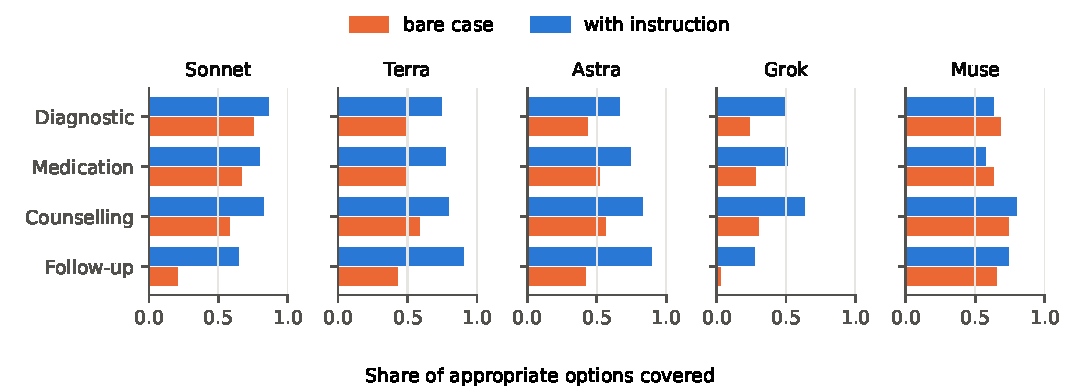
\includegraphics[width=\linewidth]{figures/fig-categories.pdf}
\caption{Share of appropriate options covered by category, bare case and with the instruction.}
\label{fig:categories}
\end{figure}

\subsection{Is the gain coverage or length?}
\label{sec:robust}
\textbf{The number of stated actions accounts for most of the effect.} In a regression of item F1 on the instruction with
model and case fixed effects (\covAdjRows{} item scores, five models), the instruction's effect was
\covAdjTotal{}. Adding the logarithm of the number of stated actions left \covAdjDirect{}: at an
equal number of stated actions, instructed and bare plans scored alike, and length accounted for
\covAdjShare\% \covAdjShareCI{} of the effect. Among the \covMatchedItems{} item pairs whose bare
and instructed plans stated within 10\% as many actions, the instructed plan scored
\covMatchedDiff{} higher on average. The instruction works largely by making models state more
actions (Figure~\ref{fig:length}). The length-only instruction (Section~\ref{sec:components}) asks
the same question by design rather than by adjustment, and qualifies the answer: at as many actions
as the plan format, it scored \covDSonnetLengthVsSpec{} for Sonnet 5.5 and \covDTerraLengthVsSpec{}
for terra against the full instruction. The count carries the effect but does not produce it alone.
Whether the added actions are worth stating is the question the next checks address.

\begin{figure}[htbp]
\centering
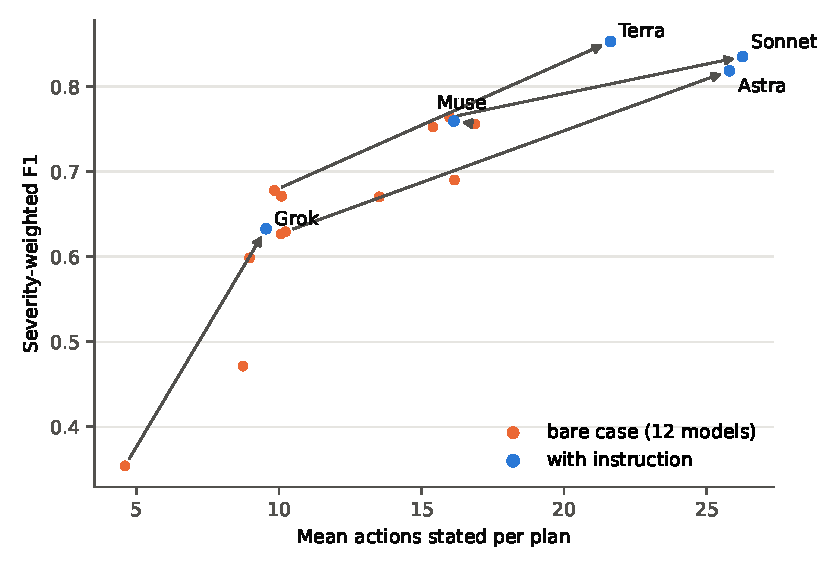
\includegraphics[width=0.78\linewidth]{figures/fig-length-f1.pdf}
\caption{Mean actions stated per plan against severity-weighted F1. Orange: the twelve models on
the bare case; blue: the five instructed arms, each joined to its bare case by an arrow.}
\label{fig:length}
\end{figure}

\textbf{Precision over every action.} The kit's headline precision ignores off-rubric actions,
which made up \covOffSonnetBare{}\% of Sonnet's bare plan and \covOffSonnetSpec{}\% of its
instructed one (Table~\ref{tab:verbosity}). Recomputed with the kit's own precision over every
stated action, where an unlisted action counts as equivocal, each gain shrank but held: Sonnet
\covDAllPromptSonnet{}, terra \covDAllPromptTerra{}, Astra \covDAllPromptAstraExh{} and Grok
\covDAllPromptGrokThorough{}. The kit's strictest variant, which counts every unlisted action as
inappropriate and weighs every option equally, reverses the gain for three models (Sonnet
\covDRawSonnet{}, terra \covDRawTerra{}, Astra \covDRawAstra{}; Grok \covDRawGrok{}); its binary
variant keeps it (Sonnet \covDBinarySonnet{}, terra \covDBinaryTerra{}). Which reading is right
depends on whether the unlisted actions are appropriate, which the rubric cannot say.

\textbf{Actions outside the rubric.} Nemotron 3 Ultra rated every unlisted action on the 90-item
sample for all four audited pairs. The instruction added unlisted actions for every model (per
item, Sonnet \covAuditActionsBareSonnet{} to \covAuditActionsPromptSonnet{}, terra
\covAuditActionsBareTerra{} to \covAuditActionsPromptTerra{}, Astra \covAuditActionsBareAstra{} to
\covAuditActionsPromptAstra{}, Grok \covAuditActionsBareGrok{} to \covAuditActionsPromptGrok{}), but
not unlisted actions rated harmful, whose number changed by \covAuditHarmDiffSonnet{},
\covAuditHarmDiffTerra{}, \covAuditHarmDiffAstra{} and \covAuditHarmDiffGrok{} per item. The rater
put \covRatedOkSonnetNemoBare--\covRatedOkTerraNemoPrompt\% of the unlisted actions in every arm at
7--9. With each unlisted action given the rater's score instead of the kit's neutral default, the
instruction's gain on the sample was \covRatedFSonnetNemo{} for Sonnet, \covRatedFTerraNemo{} for
terra, \covRatedFAstraNemo{} for Astra and \covRatedFGrokNemo{} for Grok, so by this rater's reading
the strictest variant above is the wrong one.

A second rater, Ling 3.1 Flash, rated the Sonnet pair. The two put \covAuditAgreeSonnet{} of
\covAuditAgreeActionsSonnet{} paired ratings in the same band (inappropriate, equivocal or
appropriate; Cohen's $\kappa$ \covAuditKappaSonnet{}). They differed on harm: Ling rated more of the
instructed plans' unlisted actions harmful (\covAuditHarmDiffSonnetLing{} per item), and counting an
action as harmful only when both raters did, the change was \covAuditHarmDiffSonnetBoth{}. Re-scored
with Ling's ratings, Sonnet's gain was \covRatedFSonnetLing{}. The two model raters do not agree
closely with each other, which the physician review below checks.

\textbf{Physician review.} The physician judged all \covPhysActions{} actions in Part~A
appropriate, including all \covPhysFlagged{} that a model rater had scored harmful
(\covPhysFlaggedBare{} from bare plans and \covPhysFlaggedPrompt{} from instructed ones; Nemotron
flagged \covPhysFlaggedNemo{} and Ling \covPhysFlaggedLing{}). On this sample every harm flag the
model raters raised was unfounded, so Ling's increase for Sonnet does not reflect harm the physician
recognised. The physician judged none of the \covPhysOptions{} options the specialists had rated
harmful to be harmful as the instructed plans stated them, and raised no concern with any
instruction. This is one reviewer, the study's author, giving an overall verdict, blinded in Part~A
only: a check on the model raters, not an independent clinical validation.

\textbf{Uncertainty, multiplicity and power.} Each of the four positive within-model gains had a
bootstrap $p$ below 0.001 and stayed so after Holm adjustment across the five primary contrasts
(adjusted $p$ for Sonnet \covPHolmSonnet{}, terra \covPHolmTerra{}); Muse Spark's was
\covPMuse{}. With 30 cases, the smallest difference each contrast could detect with 80\% power was
\covMdeSonnet{} for Sonnet and \covMdeTerra{} for terra.

\textbf{Evaluator consistency.} Matching the same 140 instructed terra plans twice, the primary
evaluator agreed with itself on \covRetestAgree{} of option verdicts (Cohen's $\kappa$
\covRetestKappa{}); GPT-5.6 terra agreed with it on \covCrossTerraAgree{} ($\kappa$
\covCrossTerraKappa{}) over all 330 items.

\textbf{Where the gain falls.} The gain was largest where models did worst unprompted: across the
five models, the third of cases with the lowest bare scores (mean \covTercileLowBare{}) gained
\covTercileLowGain{}, the middle third \covTercileMidGain{} and the top third (mean
\covTercileHighBare{}) \covTercileHighGain{}, consistent with a ceiling. By specialty the mean gain
ranged from \covSpecialtyMin{} (\covSpecialtyMinName) to \covSpecialtyMax{}
(\covSpecialtyMaxName), three cases each; by the kind of change a case version applies (age, sex,
medication, comorbidity and others) it ranged only from \covPerturbMin{} to \covPerturbMax{}, so the
gain does not depend on which detail of the case was perturbed. That includes the versions that
change only the patient's age (\covPerturbAge{}, \covPerturbAgeItems{} items) or sex
(\covPerturbSex{}, \covPerturbSexItems{} items), against \covPerturbBaseline{} on the original
cases, a limited check that the instruction helps regardless of these patient characteristics.

\textbf{A second evaluator.} Re-scored by Nemotron 3 Ultra, terra's gain from the instruction was
\covDPromptTerraJF{}, and the difference between the two evaluators' estimates
\covInteractionTerraJF{}; the same re-scoring of Sonnet's pair was stopped before completion and is
not reported. Under GPT-5.6
terra as evaluator, instructed terra scored \covFTerraSpecJT{} and bare Sonnet
\covFSonnetBareJT{}.

\begin{table}[htbp]
\centering\small
\caption{What the headline metric does not see. F1 (all) folds every stated action into precision;
off-rubric is the share of stated actions matching no rubric option, which the kit never scores as
harmful; worst is the mean over cases of the lowest of a case's eleven versions.}
\label{tab:verbosity}
\setlength{\tabcolsep}{4pt}
\begin{tabular}{lrrrrr}
\toprule
Configuration & F1 & F1 (all) & Off-rubric (\%) & Worst version & Median characters\\
\midrule
Sonnet 5.5, bare & \covFSonnetBare & \covFAllSonnetBare & \covOffSonnetBare & \covWorstSonnetBare & \covCharsSonnetBare\\
Sonnet 5.5, specialist & \covFSonnetSpec & \covFAllSonnetSpec & \covOffSonnetSpec & \covWorstSonnetSpec & \covCharsSonnetSpec\\
terra, bare & \covFTerraBare & \covFAllTerraBare & \covOffTerraBare & \covWorstTerraBare & \covCharsTerraBare\\
terra, specialist & \covFTerraSpec & \covFAllTerraSpec & \covOffTerraSpec & \covWorstTerraSpec & \covCharsTerraSpec\\
terra, candidate menu & \covFTerraMenu & \covFAllTerraMenu & \covOffTerraMenu & \covWorstTerraMenu & \covCharsTerraMenu\\
Astra, bare & \covFAstraBare & \covFAllAstraBare & \covOffAstraBare & \covWorstAstraBare & \covCharsAstraBare\\
Astra, exhaustive & \covFAstraExh & \covFAllAstraExh & \covOffAstraExh & \covWorstAstraExh & \covCharsAstraExh\\
Grok 4.7, bare & \covFGrokBare & \covFAllGrokBare & \covOffGrokBare & \covWorstGrokBare & \covCharsGrokBare\\
Grok 4.7, kit 500 words & \covFGrokThorough & \covFAllGrokThorough & \covOffGrokThorough & \covWorstGrokThorough & \covCharsGrokThorough\\
\bottomrule
\end{tabular}
\end{table}

\subsection{One instructed call against systems of several calls}
\label{sec:systems}
Instructed terra (one call) scored level with an ensemble of three bare plans plus a completion
pass (four calls): \covDTerraSpecVsGap{} (Table~\ref{tab:systems}). The completion pass had added
\covDGapVsUnion{} to that ensemble, so the single instruction recovers what both the second and
third models and the completion pass recovered. Concatenating the three best instructed plans
(Sonnet primary-care, terra specialist, Astra exhaustive) scored \covFUnionPrompt{}, above
instructed terra by \covDUnionPromptVsTerraSpec{}. Part of that margin is repetition: with actions
matched to the same rubric options counted once, it was \covDDedupUnionPromptVsTerraSpec{}, and
under GPT-5.6 terra as evaluator \covDDedupUnionPromptVsTerraSpecJT{}, an interval that includes
zero. Merging the concatenation into one readable plan did not work: a writer with automated
re-insertion lost source actions on the earlier, unprompted ensemble (Appendix~\ref{app:earlier}),
and on one trial item of the instructed ensemble it listed 194 source actions and lost more of
them with each repair round.

\begin{table}[htbp]
\centering\small
\caption{Single instructed calls and systems of several calls (primary evaluator unless stated).
Grouped F1 counts actions matched to the same set of rubric options once.}
\label{tab:systems}
\setlength{\tabcolsep}{4pt}
\begin{tabular}{lrll}
\toprule
Configuration & Calls & F1 [95\% CI] & Grouped F1 [95\% CI]\\
\midrule
Sonnet 5.5, bare & 1 & \covFSonnetBare{} \covCISonnetBare & \covFDedupSonnetBare{} \covCIDedupSonnetBare\\
terra, specialist & 1 & \covFTerraSpec{} \covCITerraSpec & \covFDedupTerraSpec{} \covCIDedupTerraSpec\\
Ensemble of bare Sonnet, terra, Luna & 3 & \covFUnionBare{} \covCIUnionBare & \covFDedupUnionBare{} \covCIDedupUnionBare\\
\quad + completion pass (Sonnet) & 4 & \covFGap{} \covCIGap & \covFDedupGap{} \covCIDedupGap\\
Ensemble of instructed Sonnet, terra, Astra & 3 & \covFUnionPrompt{} \covCIUnionPrompt & \covFDedupUnionPrompt{} \covCIDedupUnionPrompt\\
\quad same plans, GPT-5.6 terra as evaluator & 3 & \covFUnionPromptJT{} \covCIUnionPromptJT & \covFDedupUnionPromptJT{} \covCIDedupUnionPromptJT\\
\bottomrule
\end{tabular}
\end{table}

\subsection{Where these scores sit}
\label{sec:placement}
The benchmark publishes public-case reference scores, under its own evaluator, of 0.720 for
GPT-5.5, 0.674 for Claude Opus 4.7 and 0.664 for Gemini 3.1 Pro. The public leaderboard, scored by
the organisers on held-out cases, is led by LiSA 2.5 at 86.2, followed by Doximity Ask 6.1 (84.5)
and OpenEvidence (80.0); bare frontier models sit between about 56 and 75. Our scores are on the
public cases with a different evaluator, so none of them is a leaderboard number. NOHARM reports
that public and held-out scores correlate closely across models (Pearson 0.95)
\citep{wu2025noharm}, which supports comparing ranks, not absolute values. Two cautions apply to
absolute values here. Our second evaluator scored the instructed ensemble about 0.03 lower than the
primary one, and the primary evaluator favoured an Anthropic-written plan set by
\covJudgeInteraction{} relative to another model's in a paired test. And the public cases were
released in June 2026, so models scored afterwards may have seen them; contamination would inflate
absolute scores but not a within-model comparison of the same cases.

\FloatBarrier
\section{Discussion}
\label{sec:discussion}
On these cases an instruction did more for a model's score than the choice among the models we
tried. A plan format with a consult framing lifted terse models by as much as
\covDPromptGrokThorough{}, narrowed the field, and reordered it. The instruction's perspective and consult framing mattered
little; its plan format alone reproduced the gain, by changing how much the model stated and what. That is consistent with omission dominating NOHARM's errors: a
model that says more of what a careful specialist would do omits less, and the metric rewards
exactly that.

This extends the benchmark's own finding that priming helps generalist models
\citep{wu2025noharm}. Its priming prompts capped the answer; ours did not, and the two capped arms
here behaved differently from the uncapped ones (a large gain for the tersest model, none for one
that already wrote long plans). The cap may be part of why priming left generalists behind
clinical tools in the benchmark's report, but our data cannot separate the cap from the model.

Length is part of the mechanism, not an alternative to it. At an equal number of stated actions an
instructed plan scored no better than a bare one, so the instruction works largely by making models
say more. A count alone does not do it, though: asked only for 25 recommendations, both models
stated as many actions as under the plan format and scored below it, and Sonnet kept none of that
gain once every stated action counted in precision. The format's named contents steer which actions
are added. The question is then whether what they add is worth saying, and four checks say mostly
yes. The added actions that match the rubric are concentrated in follow-up and counselling, which
the specialists rated appropriate; counting every unlisted action in precision shrank the gains
without removing them; an independent rater put nearly all unlisted actions at 7--9 and found no
more harmful ones among them for any model, although a second rater found a small increase for
Sonnet; and the worst version of each case improved along with the average. Against that, instructed Sonnet proposed
more options the specialists rated harmful, mostly mild or moderate, and the kit's strictest
metric, which counts every unlisted action as wrong, reverses the gain for three models.
Under an evaluator from a third model family, Nemotron 3 Ultra, terra's gain was
\covDPromptTerraJF{}, within \covInteractionTerraJF{} of the primary estimate.
The author, a physician, then read every unlisted action a model rater had flagged and every
harmful option an instruction added, and judged none harmful as stated. One reviewer's overall
verdict, blinded only for the unlisted actions, is not a panel's item-level ratings, and AI
evaluators are known to favour longer text
\citep{zheng2023judging,saito2023verbosity,dubois2024length}. The safest reading is that the
instruction makes models state more of the indicated actions, along with a few options the
benchmark's specialists rated harmful in general that one physician did not find harmful in
context, and that under the benchmark's severity weighting the first outweighs the second.

Two practical consequences follow. For benchmark design, an unprompted protocol ranks a model
partly on its default verbosity; reporting prompted and unprompted results, as NOHARM's own study
does, makes that visible, and so does reporting how much a model's score depends on actions the
rubric cannot see. For system design, a single instructed call matched a four-call ensemble with
completion at a quarter of the calls, taking a median of \covRuntimeTerraSpec{} seconds per case
(90th percentile \covRuntimePninetyTerraSpec{}) against the benchmark's 300-second limit; combining
instructed models added a little more, with an uncertain margin under a second evaluator. Neither
result says anything about clinical usefulness: a plan of twenty to thirty items needs ordering by
priority before a clinician can use it.

The intended use the benchmark represents is advice to a primary-care clinician who has asked a
specialist about one patient: the input is the clinician's question with the case details, the
output a management plan that the clinician reads, judges and acts on. Nothing here evaluates a
plan acting without that clinician, and the instruction is only as safe as the reader of a longer
plan is attentive.

Four next steps would turn these observations into tests. Scoring instructed and bare models on
the held-out cases would show whether the gain survives the organisers' evaluator on unseen cases;
the public leaderboard admits distinct models rather than prompts, so this needs the organisers'
own runs or a research arrangement with them. A blinded panel rating the added actions item by
item, as the benchmark's specialists rated its rubric, would turn this study's single-reviewer check
into a measurement. Giving one instruction to every model, testing the length cap within a model and measuring
regeneration noise would remove the remaining confounds in this design. And reporting prompted
beside unprompted scores on other clinical benchmarks would show whether the gap between general
models and clinical tools is a property of the models or of how they are asked.

\section{Limitations}
\label{sec:limitations}
\textbf{Small development set.} The study has \nCases{} base cases, not \nItems{} independent
consultations, and instructions and systems were developed on these same cases; although none
names a rubric option, estimates may be optimistic.

\textbf{An incomplete design.} Five of twelve models were instructed, with different instructions,
and cross-model statistics rest on those five. The instruction's parts were separated on two models
only. The capped and uncapped instructions went to different models, so the cap's own effect is
untested. Regeneration noise was not measured; evaluator noise was, on one arm. Several planned arms
were stopped before completion and are not analysed.

\textbf{Automated evaluation.} Every score comes from an AI evaluator, not the organisers' and not
physicians. A second family re-scored the key contrasts. The author, an internal-medicine
physician, reviewed the off-rubric actions the model raters flagged, the harmful options the
instruction added and the instructions, giving an overall verdict rather than item-level scores,
blinded only for the off-rubric actions. No physician reviewed whole plans or evaluator
disagreements, and no independent panel was used.

\textbf{What the metric cannot see.} Headline precision ignores actions the rubric does not list,
and the kit never counts them as harmful; our checks bound this but do not replace clinical review.
Longer plans may also be harder to use; usability was not measured.

\textbf{Contamination and drift.} The public cases have been available since June 2026. Provider
routes and model versions change, and free models may retain inputs.

\section{Conclusion}
\label{sec:conclusion}
A structured, uncapped instruction raised NOHARM scores for every terse model we tested, narrowed
the gap between models, and matched a multi-model system with one call, through stating more of the
indicated actions. Benchmarks of clinical completeness should report prompted beside unprompted
results, and comparisons between models, or between models and clinical tools, should be made
under both before conclusions are drawn.

\section*{Data, code, and declarations}
\textbf{Reproducibility.} The offline analysis is \nolinkurl{scripts/noharm_paper_snapshot.py}; it
hashes every source file, refuses an incomplete arm, and writes every number in this manuscript to
\nolinkurl{docs/paper/coverage-numbers.tex}. Instructions are in
\nolinkurl{scripts/noharm_system.py}; the off-rubric audit is
\nolinkurl{scripts/noharm_offrubric_audit.py}. Every model response, evaluation, rating, the
physician review materials and the code are archived at
\url{https://github.com/OJamals/noharm-prompting} (code MIT, data CC BY 4.0); the generators
reproduce every number in this manuscript from that archive without model calls.

\textbf{Ethics and data use.} The study reused public benchmark data and involved no patient
intervention. The NOHARM v2 public cases are released under CC BY 4.0 and contain no identifiable
patient information, and the only person involved was the author, as physician reviewer; the study
uses only openly available data, is not human-subjects research, and was not submitted for ethics
review. All materials
produced here are released openly, without access restrictions.

\textbf{Protocol, registration and involvement.} No protocol was prepared and the study was not
registered; it is an exploratory analysis of development data (Section~\ref{sec:statistics}). No
patients or members of the public were involved in its design, conduct or reporting.

\textbf{Reporting.} The TRIPOD-LLM checklist \citep{gallifant2025tripodllm} for this study is in
Appendix~\ref{app:tripod}.

\textbf{Author contributions.} Ahmad Omar Aljamal designed the study, directed the experiments and
analysis, performed the physician review, and is responsible for the manuscript.

\textbf{Funding.} This work received no funding. Neither the author nor any institution received
payment or services from a third party for any aspect of it.

\textbf{Competing interests.} The author declares no competing interests, and has received no
payments or services from a third party in the past 36 months that could be perceived to influence,
or give the appearance of influencing, this work.

\textbf{AI assistance.} Experiments, analysis and drafting were assisted by Claude Code and
Codex; earlier drafting used the Scientific Agent Skills workflow \citep{kassis2026skills}. AI
systems are not authors. The author reviewed the manuscript, references and declarations and takes
responsibility for them.

\begingroup
\small
\setlength{\bibsep}{0.4\baselineskip}
\bibliographystyle{plainnat}
\bibliography{refs}
\endgroup

\clearpage
\appendix
\section{Instructions, verbatim}
\label{app:prompts}
In every instruction below, \texttt{\{case\}} stands for the item's case text. The bare condition
sends the case text alone.

\textbf{Consult framing} (\texttt{SPECIALIST}):
\begin{lstlisting}
A primary care colleague has consulted you, a specialist, about the case below. Work only with the information provided. Give the best recommendations for the situation, not only an answer to the literal question.
\end{lstlisting}

\textbf{Plan format} (\texttt{PLAN\_FORMAT}):
\begin{lstlisting}
Start with a one- or two-sentence clinical assessment, then give your recommendations as numbered items. Be specific: exact tests, drugs with doses and durations, referral specialty and urgency, conditional next steps, case-specific counseling, and return precautions. Include every action a careful specialist would not want omitted; include nothing unsafe or unwarranted.
\end{lstlisting}

\textbf{Specialist}: \texttt{SPECIALIST}, a blank line, \texttt{Case:} and the case, a blank line,
\texttt{PLAN\_FORMAT}.

\textbf{Components}: \emph{framing only} is \texttt{SPECIALIST}, a blank line, \texttt{Case:} and
the case. \emph{Format only} is \texttt{Case:} and the case, a blank line, \texttt{PLAN\_FORMAT}.
\emph{Length only} is \texttt{Case:} and the case, a blank line, then:
\begin{lstlisting}
Respond with at least 25 numbered recommendations.
\end{lstlisting}

\textbf{Exhaustive headings}: \texttt{SPECIALIST} extended as below, then the case and
\texttt{PLAN\_FORMAT}:
\begin{lstlisting}
Address each of these headings for THIS patient, and write 'none indicated' under a heading only after considering it: diagnosis and its severity; tests to confirm, to exclude dangerous alternatives, and baselines before treatment; medications to start, stop, hold or adjust (drug, dose, route, duration) and interactions with current ones; procedures; referrals (specialty, urgency); counseling and warning signs; follow-up and monitoring (what, when, who); contingencies (if X, then Y, with thresholds).
\end{lstlisting}

\textbf{Perspectives}, each followed by the case and \texttt{PLAN\_FORMAT}:
\begin{lstlisting}
You are a clinical pharmacist on the consulting team for the case below. Work only with the information provided. Give the complete management plan, paying particular attention to every medication that should be started, stopped, held or adjusted (drug, dose, route, duration), interactions with the current regimen, renal or hepatic dosing, prophylaxis, and the monitoring each drug needs.
\end{lstlisting}
\begin{lstlisting}
You are the patient's primary care physician, responsible for carrying out the plan for the case below over the coming months. Work only with the information provided. Give the complete management plan, paying particular attention to follow-up (what, when, who), contingencies with explicit thresholds (if X, then Y), what the patient must be told and watch for, and the referrals with their urgency.
\end{lstlisting}

\textbf{Candidate menu}: a request to list every concrete action a specialist panel should
consider, alternatives and debatable actions included, under named headings, aiming for 30--50
numbered actions without marking any as recommended; full text in
\nolinkurl{scripts/noharm_system.py} (\texttt{MENU}).

\textbf{Kit thorough prompt.} The NOHARM kit's \texttt{prompts/thorough.md}, used unmodified: a
consult framing, a request for a brief assessment and numbered recommendations under 500 words,
the criteria completeness, safety and restraint, and a list of what a response may cover.

\textbf{Completion pass}: \texttt{SPECIALIST}, the case and the source plans, then a request to
list only clearly indicated actions none of the plans states, checked heading by heading
(follow-up and monitoring, contingencies, medications, diagnostics, referrals and procedures,
counselling), as numbered concrete actions or ``No additions.''; full text in
\nolinkurl{scripts/noharm_system.py} (\texttt{GAP}).

\section{Technical and statistical details}
\label{app:technical}
\textbf{Kit and evaluator.} We used the NOHARM kit from the MAST repository at revision
\texttt{57a12c5490f3a7a6b0a6ce4e0d49f8e393ff49ee} (code MIT, data CC BY 4.0), its runner, match and
review stages and metric code unchanged. Only the evaluator model was replaced, because the
organisers' evaluator family was outside the models available to us. The evaluator receives the
kit's JSON schema in its prompt and its reply is validated locally. Model identifiers name provider
routes, not immutable checkpoints. The free evaluators were reached through OpenRouter at zero
price (Nemotron 3 Ultra, \texttt{nvidia/nemotron-3-ultra-550b-a55b:free}; Ling 3.1 Flash,
\texttt{inclusionai/ling-3.1-flash}), with the public cases only, because free routes may retain
prompts.

\textbf{Generation.} Instructed and system calls requested temperature zero and at most 12,000
output tokens, with up to four attempts for transient failures or empty replies; routes could
ignore temperature. Bare and kit-prompt arms used the kit's runner and defaults. An arm is analysed
only when all \nItems{} items have a non-empty response and a complete evaluation; incomplete arms
are excluded, never scored as answers. Responses were used as returned: no post-processing other than
the concatenation that defines an ensemble, and no item was edited or filtered.

\textbf{Dates and versions.} All analysed generations and evaluations were run between
\covFirstJudged{} and \covLastJudged{}. Models were reached through provider routes whose names
are given in Section~\ref{sec:models}; the routes expose neither an immutable checkpoint nor a
training cut-off date, so neither is reported, and a later run of the same route may differ.

\textbf{Compute.} Every model call went to a provider's hosted service; no local training or
inference was run. An arm is \nItems{} generation calls and about two evaluation calls per item
(matching and review). Instructed terra took a median of \covRuntimeTerraSpec{} seconds per item
(90th percentile \covRuntimePninetyTerraSpec{}), bare terra \covRuntimeTerraBare{}. Commercial
models were reached through subscription accounts behind a local gateway, whose per-call cost is not
itemised; the freely available models, the second evaluator and the audit raters were reached at
zero price.

\textbf{Metric.} Rubric options are rated inappropriate (1--3), equivocal (4--6) or appropriate
(7--9), with severity weights 72, 24 and 3 for the outer, middle and inner scores and 1 for
equivocal options. The kit handles partial matches, alternative options and dependencies. Its
off-rubric-inclusive precision gives each unmatched action the neutral default score.

\textbf{Grouped scores.} Actions matched to the same set of rubric options are collapsed and the
kit's metric code rescores the plan; both sides of a comparison receive the same transformation.
Distinct recommendations can share an option set, so grouping is a sensitivity analysis, not an
alternative metric.

\textbf{Resampling.} For case scores $f_{ia}$ the paired difference is
$\widehat{\Delta}_{b-a} = N^{-1}\sum_{i=1}^{N}(f_{ib}-f_{ia})$ with $N=\nCases$. Cases were
resampled with replacement, unstratified, 10,000 times with seed 7; cross-model statistics
(Spearman, standard deviation, range, Kendall's $\tau$) are recomputed on each resample.

\section{Earlier experiments on unprompted plans}
\label{app:earlier}
Before the instruction experiments, we combined bare plans from Sonnet 5.5, terra and Luna. The
ensemble scored \covFUnionBare{} (\covDUnionBareVsSonnet{} over bare Sonnet); a Sonnet completion
pass raised it to \covFGap{} (\covDGapVsUnion{}), and Opus 5.5 in the same role changed nothing
(\covDOpusVsSonnetGap{}). A writer with automated omission checks scored \covFWriterBare{}
(\covDWriterVsUnion{} against the ensemble), but its checker still reported a mean of
\covMissingFinalMean{} of a median \covSourceActionsMedian{} source actions missing after repair,
so the rewrite was not lossless. On the instructed ensemble, a trial of the same writer on one
item listed 194 source actions, and its re-insertion rounds left more of them missing each round.

\section{TRIPOD-LLM checklist}
\label{app:tripod}
Reporting follows TRIPOD-LLM \citep{gallifant2025tripodllm}. Item topics are paraphrased; the
guideline gives their full wording. The study's research designs are prompt engineering (M) and
LLM evaluation (E), and its task is long-form question answering (QA), so items restricted to other
designs or tasks are marked not applicable (N/A). ``Sec.'' and ``App.'' refer to this manuscript.

{\small
\setlength{\tabcolsep}{4pt}
\renewcommand{\arraystretch}{1.12}
\begin{longtable}{>{\raggedright\arraybackslash}p{0.06\linewidth}
  >{\raggedright\arraybackslash}p{0.33\linewidth}
  >{\raggedright\arraybackslash}p{0.53\linewidth}}
\toprule
Item & Topic & Where reported, or response\\
\midrule
\endfirsthead
\toprule
Item & Topic & Where reported, or response\\
\midrule
\endhead
\multicolumn{3}{l}{\textit{Title and abstract}}\\
1 & Study type, task, population, outcome in the title & Title: language models, prompt design,
  a clinical-safety benchmark of specialist consultations; subtitle names the NOHARM v2 public cases.\\
2 & Structured abstract (TRIPOD-LLM for abstracts) & Abstract: background, objective, methods,
  results with intervals, conclusions.\\
\multicolumn{3}{l}{\textit{Introduction}}\\
3a & Healthcare context, rationale, existing approaches & Sec.~\ref{sec:intro},
  Sec.~\ref{sec:related}.\\
3b & Target population, intended use and users & Sec.~\ref{sec:intro}; intended use stated in
  Sec.~\ref{sec:discussion} (advice to a primary-care clinician, reviewed before action).\\
4 & Objectives and study stage & Sec.~\ref{sec:intro}: four questions; evaluation of existing models
  under different instructions; no development or tuning.\\
\multicolumn{3}{l}{\textit{Methods}}\\
5a & Data sources and rationale & Sec.~\ref{sec:benchmark}.\\
5b & Description and distribution of the data & Sec.~\ref{sec:benchmark}: cases, specialties,
  versions, rubric composition by score and category.\\
5c & Dates of the oldest and newest text & Public cases released June 2026
  (Sec.~\ref{sec:placement}); the benchmark does not date the source consultations. Training-data
  dates of the models are not available (App.~\ref{app:technical}).\\
5d & Preprocessing and quality checks & App.~\ref{app:technical}: cases sent verbatim; completeness
  checks; re-scored plans verified byte-identical.\\
5e & Missing and imbalanced data & App.~\ref{app:technical}: incomplete arms excluded, undefined
  precision handled as in the kit; categories with too few options not reported
  (Sec.~\ref{sec:mechanism}).\\
6a & Model name, version, training date & Sec.~\ref{sec:models}; App.~\ref{app:technical}: provider
  routes, no immutable checkpoint or training cut-off available.\\
6b & Model development process & N/A: existing models used without training or tuning.\\
6c & Generation details: prompts, inference settings, consistency & Sec.~\ref{sec:prompts};
  App.~\ref{app:prompts} (verbatim); App.~\ref{app:technical} (temperature, tokens, retries).
  Regeneration consistency not measured (Sec.~\ref{sec:limitations}).\\
6d & Raw and post-processed output & App.~\ref{app:technical}: unstructured text, used as returned.\\
6e & Classification thresholds & N/A (task is long-form question answering).\\
7a & Output-quality metrics against a gold standard & Sec.~\ref{sec:outcomes}: severity-weighted F1
  against specialist ratings, with precision, recall, severe-error share and four length checks.\\
7b & Metric relevance; correlation with human evaluation & Sec.~\ref{sec:evaluation}: evaluator
  agreement with the organisers' evaluator; one physician's overall review of flagged unlisted
  actions and added harmful options (Sec.~\ref{sec:robust}, Sec.~\ref{sec:limitations}).\\
7c & Outcome definition, calculation, inference dates & Sec.~\ref{sec:outcomes};
  App.~\ref{app:technical} (kit revision, metric code, dates).\\
7d & Subjective assessment: assessors, instructions, agreement & AI evaluators with the kit's
  prompts (Sec.~\ref{sec:evaluation}); test--retest and cross-family agreement
  (Sec.~\ref{sec:robust}).\\
7e & Comparison with other models, humans, benchmarks & Twelve models (Sec.~\ref{sec:grid});
  published reference and leaderboard scores (Sec.~\ref{sec:placement}); no human comparison.\\
8a & Annotation process & Rubric rated by the benchmark's specialists \citep{wu2025noharm};
  off-rubric actions rated by models on the same 1--9 scale (Sec.~\ref{sec:outcomes}).\\
8b & Annotators, overlap, agreement & Two model raters on a shared 90-item sample
  (Sec.~\ref{sec:robust}).\\
8c & Annotator background or labelling-model characteristics & Sec.~\ref{sec:outcomes}: rater
  models and their accuracy against specialist ratings in an earlier analysis.\\
9a & Prompt design, curation and selection & Sec.~\ref{sec:prompts}.\\
9b & Data used to develop prompts & Sec.~\ref{sec:prompts}: the same public cases
  (Sec.~\ref{sec:limitations}).\\
10 & Preprocessing before summarisation & N/A (task is not summarisation).\\
11 & Instruction tuning or alignment & N/A (no tuning).\\
12 & Compute & App.~\ref{app:technical}: hosted calls, calls per arm, runtimes.\\
13 & Ethics approval & Not human-subjects research; public CC BY 4.0 cases, no review sought
  (Data, code and declarations).\\
\multicolumn{3}{l}{\textit{Open science and involvement}}\\
14a & Funding & None (Data, code and declarations).\\
14b & Conflicts of interest & None (Data, code and declarations).\\
14c & Protocol & No protocol prepared (Data, code and declarations).\\
14d & Registration & Not registered (Data, code and declarations).\\
14e & Data availability & Responses, evaluations and analysis outputs; archive
  \url{https://github.com/OJamals/noharm-prompting}.\\
14f & Code availability & Analysis and generation scripts named in Data, code and declarations;
  archive \url{https://github.com/OJamals/noharm-prompting}.\\
15 & Patient and public involvement & None (Data, code and declarations).\\
\multicolumn{3}{l}{\textit{Results}}\\
16a & Flow of data through the study & Sec.~\ref{sec:benchmark}: \nCases{} cases, \nItems{} items,
  all analysed in every complete arm; no patient-level data.\\
16b & Characteristics per data source and split & N/A: no development/evaluation split; case
  composition in Sec.~\ref{sec:benchmark}.\\
16c & Clinical-variable distribution, development vs.\ evaluation & N/A (no split, no clinical
  outcomes).\\
16d & Numbers in each analysis & \nItems{} items per arm; 90-item audit sample; 140-item test--retest
  (Sec.~\ref{sec:robust}).\\
17 & Performance on prespecified metrics & Sec.~\ref{sec:grid}--\ref{sec:placement}.\\
18 & Model updating & N/A: no updating; provider routes may change (Sec.~\ref{sec:limitations}).\\
\multicolumn{3}{l}{\textit{Discussion}}\\
19a & Interpretation, including fairness & Sec.~\ref{sec:discussion}; age and sex versions
  (Sec.~\ref{sec:robust}).\\
19b & Limitations & Sec.~\ref{sec:limitations}.\\
19c & Data challenges: representation, missingness, bias & Sec.~\ref{sec:limitations}: one centre,
  30 cases, public since June 2026.\\
19d & Intended use, input, user, autonomy & Sec.~\ref{sec:discussion}.\\
19e & Handling poor or missing input & N/A in a benchmark; robustness across case versions
  (Sec.~\ref{sec:robust}).\\
19f & User interaction and expertise & Sec.~\ref{sec:discussion}: a longer plan needs prioritising
  for a clinician reader.\\
19g & Next steps & Sec.~\ref{sec:discussion}, Sec.~\ref{sec:conclusion}.\\
\bottomrule
\end{longtable}
}
\end{document}
